\chapter{\iftoggle{german}{Verwandte Arbeiten}{Related Work}}\label{ch:related_work}

This chapter discusses the previous contributions to indoor synthetic datasets in ~\autoref{subsec:indoor-synthetic-datasets},
what tasks each dataset supports, and some disadvantages.
Further, we discuss the available tools which support the creation of indoor dataset~\autoref{subsec:tools-to-create-synthetic} on different platforms and frameworks.
~\autoref{sec:state_of_the_art} will contain state-of-the-art 3D Reconstruction techniques used with different model representations(Voxels, Mesh, Point Clouds).
We will also discuss ways to mitigate the domain gap in ~\autoref{sec:mitigating_domain_shift}.
This section will include traditional techniques like transfer learning or fine-tuning and mixed training.
Recent trends in Generative models to transfer the style of the real image onto synthetically generated images is also briefly discussed.


\section{Indoor datasets}\label{sec:indoor-dataset}

Indoor scene dataset has been in the rise with increasing interest in scene processing understanding~\cite{dai2017scannet,Silberman2012IndoorSA,Xiao2013SUN3DAD,Hua2016SceneNNAS,Armeni20163DSP,chang2017matterport3d,Handa2016UnderstandingRI,InteriorNet18,li2021openrooms,zheng2020structured3d,Roberts2020HypersimAP,McCormac:etal:ICCV2017}.
The use of synthetic datasets is not something new in the world of machine learning.
As researchers realized the disadvantages of a real dataset, the focus shifted towards the synthetic dataset.
While~\cite{dai2017scannet} are real-world datasets,~\cite{Fu20203DFRONT3F,Handa2016UnderstandingRI,McCormac:etal:ICCV2017,Roberts2020HypersimAP} are synthetically produced.
Live scans help to gather real-world datasets.
The synthetic dataset can be manually configured by a professional or automated by a programmer using a tool.

\subsection{Indoor synthetic datasets}\label{subsec:indoor-synthetic-datasets}
Alibaba group introduced \gls{front}~\cite{Fu20203DFRONT3F} which stands for 3D Furnished Rooms with layOuts and semaNTics dataset which comprises
synthetic indoor scenes designed under the supervision of professionals.
It consists of 18,968 rooms and 13,151 textured pieces of furniture.
SceneNet~\cite{McCormac:etal:ICCV2017} is an extensive collection of photorealistic images and trajectories.
We will discuss this dataset in detail in~\autoref{sec:role-of-scenenet}.

SunCG~\cite{Song2017SemanticSC} was a fundamental dataset for scene understanding.
The dataset contained over 45,000 variations of scenes with realistic room layouts created manually.
Each scene was semantically labeled and also provided with volumetric ground truth data.
We use the dataset for tasks like depth estimation, semantic scene completion, SLAM, indoor navigation, and more.
Unfortunately, due to legal issues \footnote{https://futurism.com/tech-suing-facebook-princeton-data} the dataset has been made publicly unavailable, leaving a void in the field.

Structure3D~\cite{zheng2020structured3d} is another impressive synthetic data for indoor scenes which introduced their own photorealistic renderer.
The dataset comprises 21,835 rooms in 3,500 scenes and 196k 2D images rendered with photorealism.
However, the CAD models of the 3D furniture used to populate the scenes are not made available to the public.
Hence, we cannot perform the tasks related to  3D reconstruction.
\cite{zheng2020structured3d} have also demonstrated that combining synthetic and real dataset deep learning tasks for room layout estimation improved performance on benchmark datasets.
This dataset focuses more on room layout estimation and not 3D reconstruction, but with few modifications, it may well support to 3d furniture reconstruction tasks.

Openrooms~\cite{li2021openrooms} use Scannet~\cite{dai2017scannet} as their layout foundation, retrieve corresponding models from shapenet~\cite{chang2015shapenet}
and then replace the CAD model with a retrieved model with proper alignment.
They further add the reflectance and illumination properties to compose photo-realistic images.
As of August 2021, only the dataset has been made public, not the generation tool or CAD models.
The underlying concept of Openrooms is to convert existing scans into photorealistic synthetic images.
We consider them our counterparts in the output images, as the framework can produce normals, depth maps, instance segmentation, and masks the same as we do.

Hypermism~\cite{Roberts2020HypersimAP} is Apple's repository for holistic indoor scene understanding.
It is a collection of synthetic scenes created with the help of a professional artist.
Evermotion ~\cite{Evermotion} was the starting point for the dataset for which assets were purchased from TurboSquid~\cite{TurboSquid}.
The dataset includes images, 3D assets, semantic instance segmentation, and a disentangled image representation with diffused lighting and shading.
Even though the 3d triangle meshes for each asset is available online, we have to purchase them to create a custom dataset.
They also admit that the cost to generate the dataset is expensive \{approximately \$57K~\cite{Roberts2020HypersimAP}\}.

InteriorNet~\cite{InteriorNet18} claims to be a photo-realistic indoor scene simulator with realistic lighting and scenes which change over time.
The image dataset includes RGB, depth, and semantic segmentation.
Along with images, they also provide synthesized realistic trajectories at a video-frame rate with various motion patterns.
The simulator also supports scenes from~\cite{McCormac:etal:ICCV2017} and~\cite{Song2017SemanticSC} along with their database.

Another simulated framework for visual research is House Of inteRactions (THOR) was introduced in \gls{ai2thor}~\cite{kolve2019ai2thor}.
This dataset is again an Agent focused photo-realistic dataset with the critical factor being actionable objects so that agents can interact with the objects or manipulate them.
The underlying renderer for this framework is the Unity game engine.
RoboThor~\cite{Deitke2020RoboTHORAO} is built upon \gls{ai2thor}, consisting of real scenes and its corresponding synthetic equivalent.
It helps study agents' behavior in the real world when trained on synthetic data.
Architects manually designed the scenes by taking references from photos of the real world.

Habitat: A Platform for Embodied AI Research~\cite{savva2019habitat} is a photorealistic 3D simulation used for training virtual agents for tasks like navigation, question answering, instruction following..
The paper introduces Habitat-Sim, which renders scenes from Matterport3d~\cite{chang2017matterport3d}, Gibson~\cite{xia2018gibson}, Replica~\cite{Straub2019TheRD}, and some other datasets.
The focus of the simulator is providing the agent with sensor data and allowing additional sensors as plugins.
At the foundation level, Habitat-sim uses Magnum graphics
middleware library~\footnote{https://magnum.graphics/}, which supports cross-platform on the various hardware configuration.

In \autoref{fig:photorealistic images comparison}, we can see samples from each of the datasets claimed to be photorealistic.
The images from these datasets are used in a research survey to determine the perception of humans about photorealism.
We define "Automated dataset" as a dataset which had no or limited user or professional designer inputs.
Only the 3D furntiure models assets might have been designed by professionals, but the properties of the room like lights, textures, etc, were generated automatically.
Among the datasets under consideration,
OpenRooms, SceneNet, BlenderProc are all automated datasets, including the proposed \gls{free} dataset.
Hyperism, \gls{ai2thor}, InteriorNet, and \gls{front} were manually configured and designed by professional architects.


\begin{table}[ht]
    \centering
    \begin{tabular}{|c |c |c |c|}
        \hline
        Dataset & Year & Automated \\ [0.5ex]
        \hline\hline
        Openrooms & 2020 & YES \\
        \hline
        \gls{ai2thor} & 2017 & NO \\
        \hline
        BlenderProc & 2019 & YES \\
        \hline
        Hyperism & 2020 & NO \\
        \hline
        \gls{front} & 2020 & NO \\
        \hline
        InteriorNet & 2018 & NO \\
        \hline
        SceneNet & 2015 & YES \\
        \hline
        \gls{free} & 2021 & YES \\[1ex]
        \hline
    \end{tabular}
    \caption{Table represents synthetic datasets and year of release, and if they are automated(i.e. created with no or limited inputs from professional designers.)}
    \label{tab:dataset_comparison}
\end{table}

\begin{figure}
\begin{tabular}{llll}
    \gls{front} & 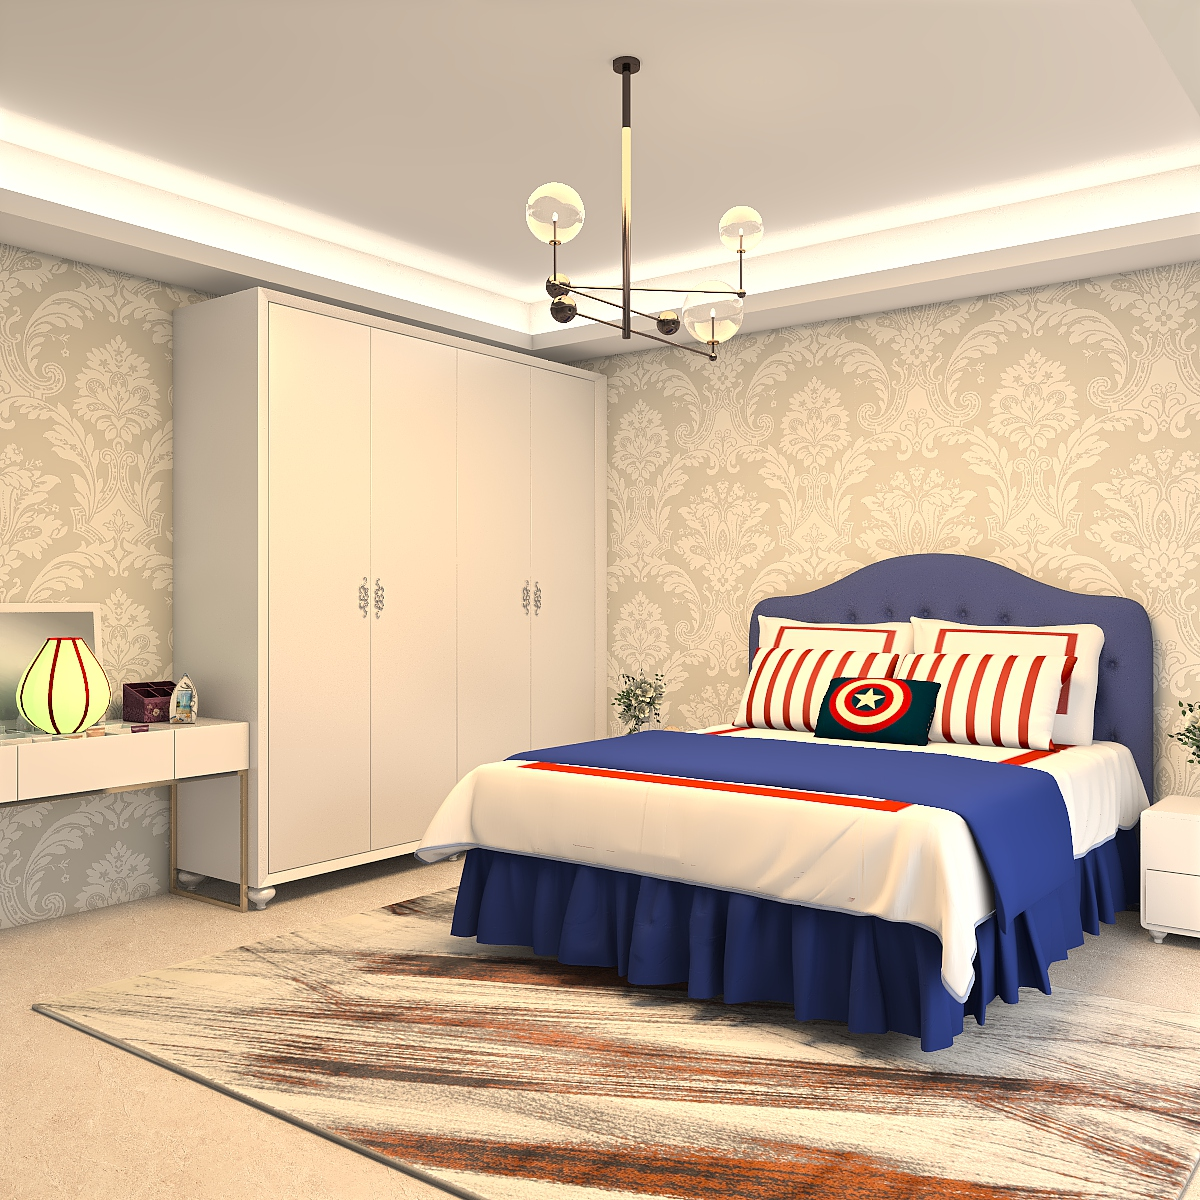
\includegraphics[width=.2\linewidth,valign=m]{/Users/apple/OVGU/Thesis/code/3dReconstruction/report/images/realistic_images_relatedwork/3dfront_1} &
    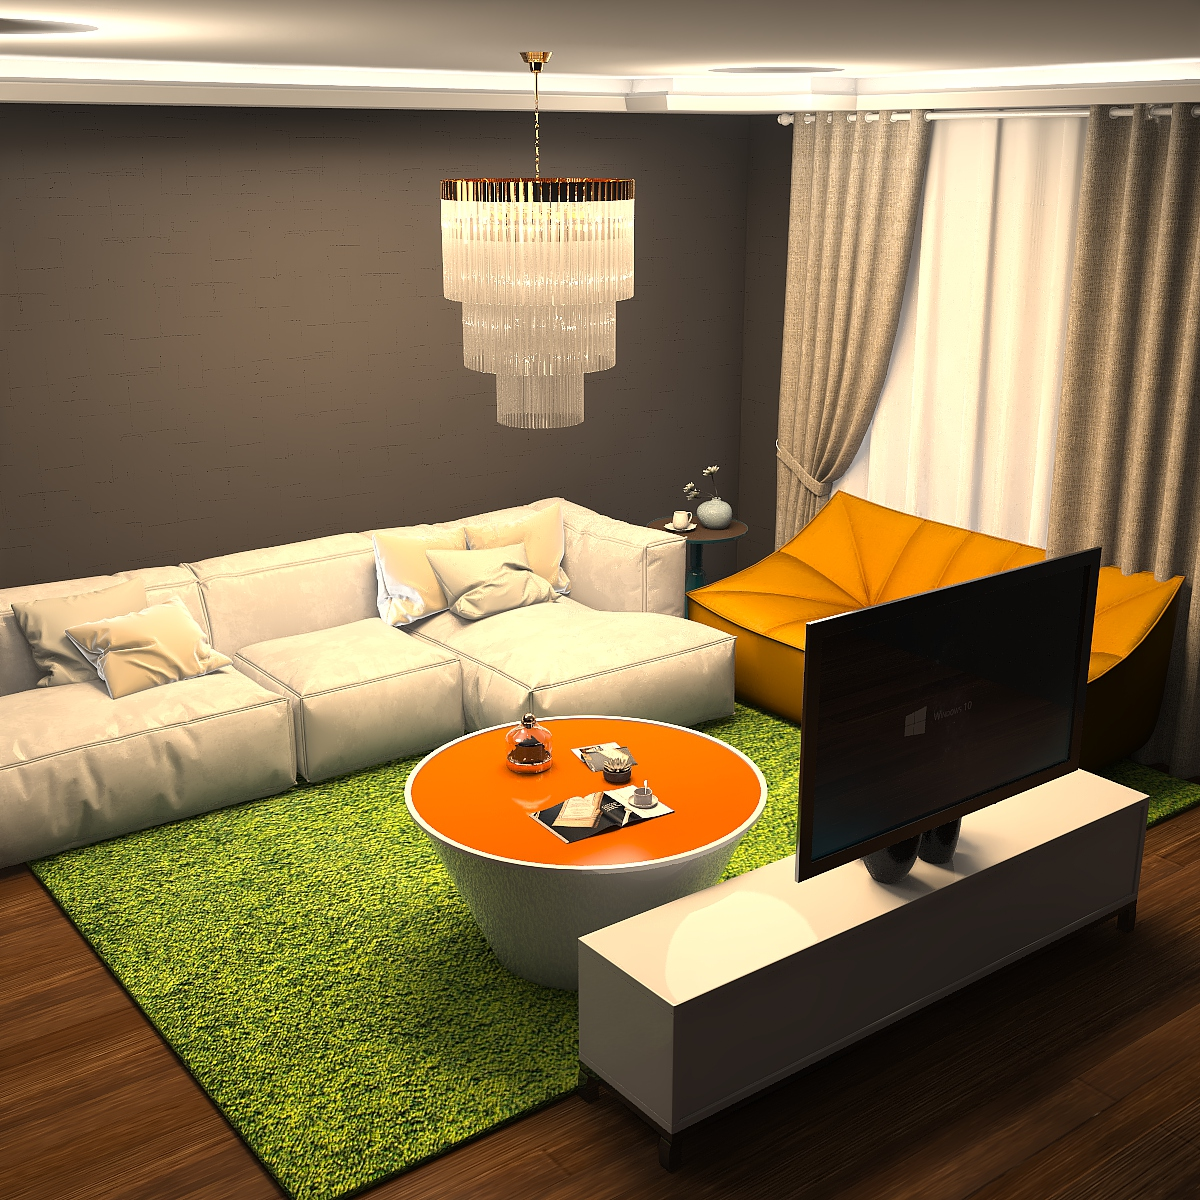
\includegraphics[width=.2\linewidth,valign=m]{/Users/apple/OVGU/Thesis/code/3dReconstruction/report/images/realistic_images_relatedwork/3dfront_2} &
    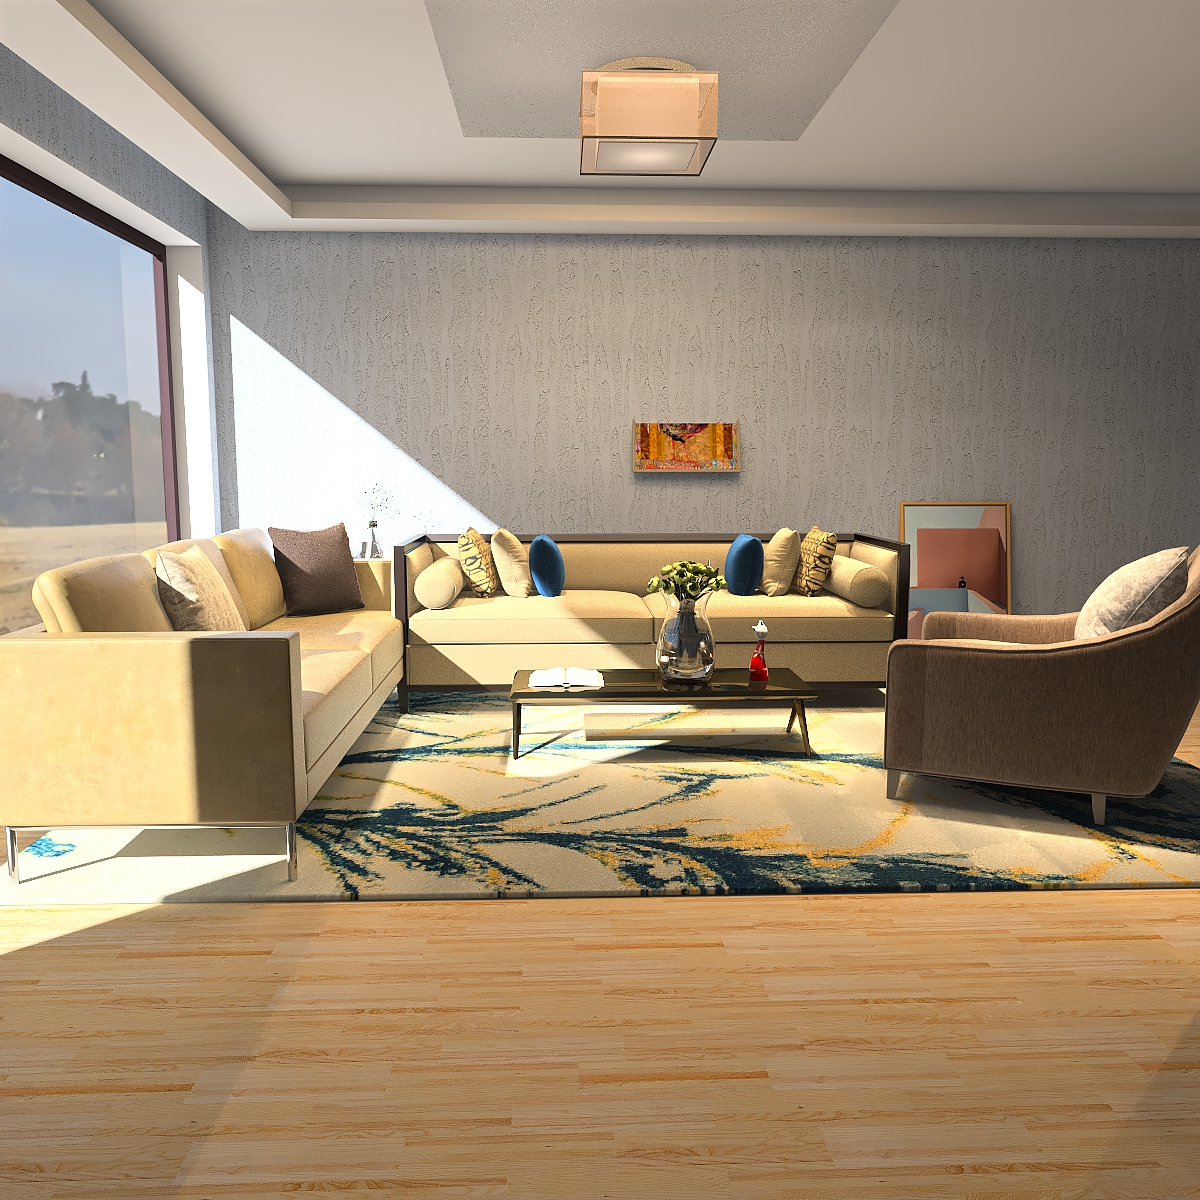
\includegraphics[width=.2\linewidth,valign=m]{/Users/apple/OVGU/Thesis/code/3dReconstruction/report/images/realistic_images_relatedwork/3dfront_3}\\

    \gls{ai2thor} & 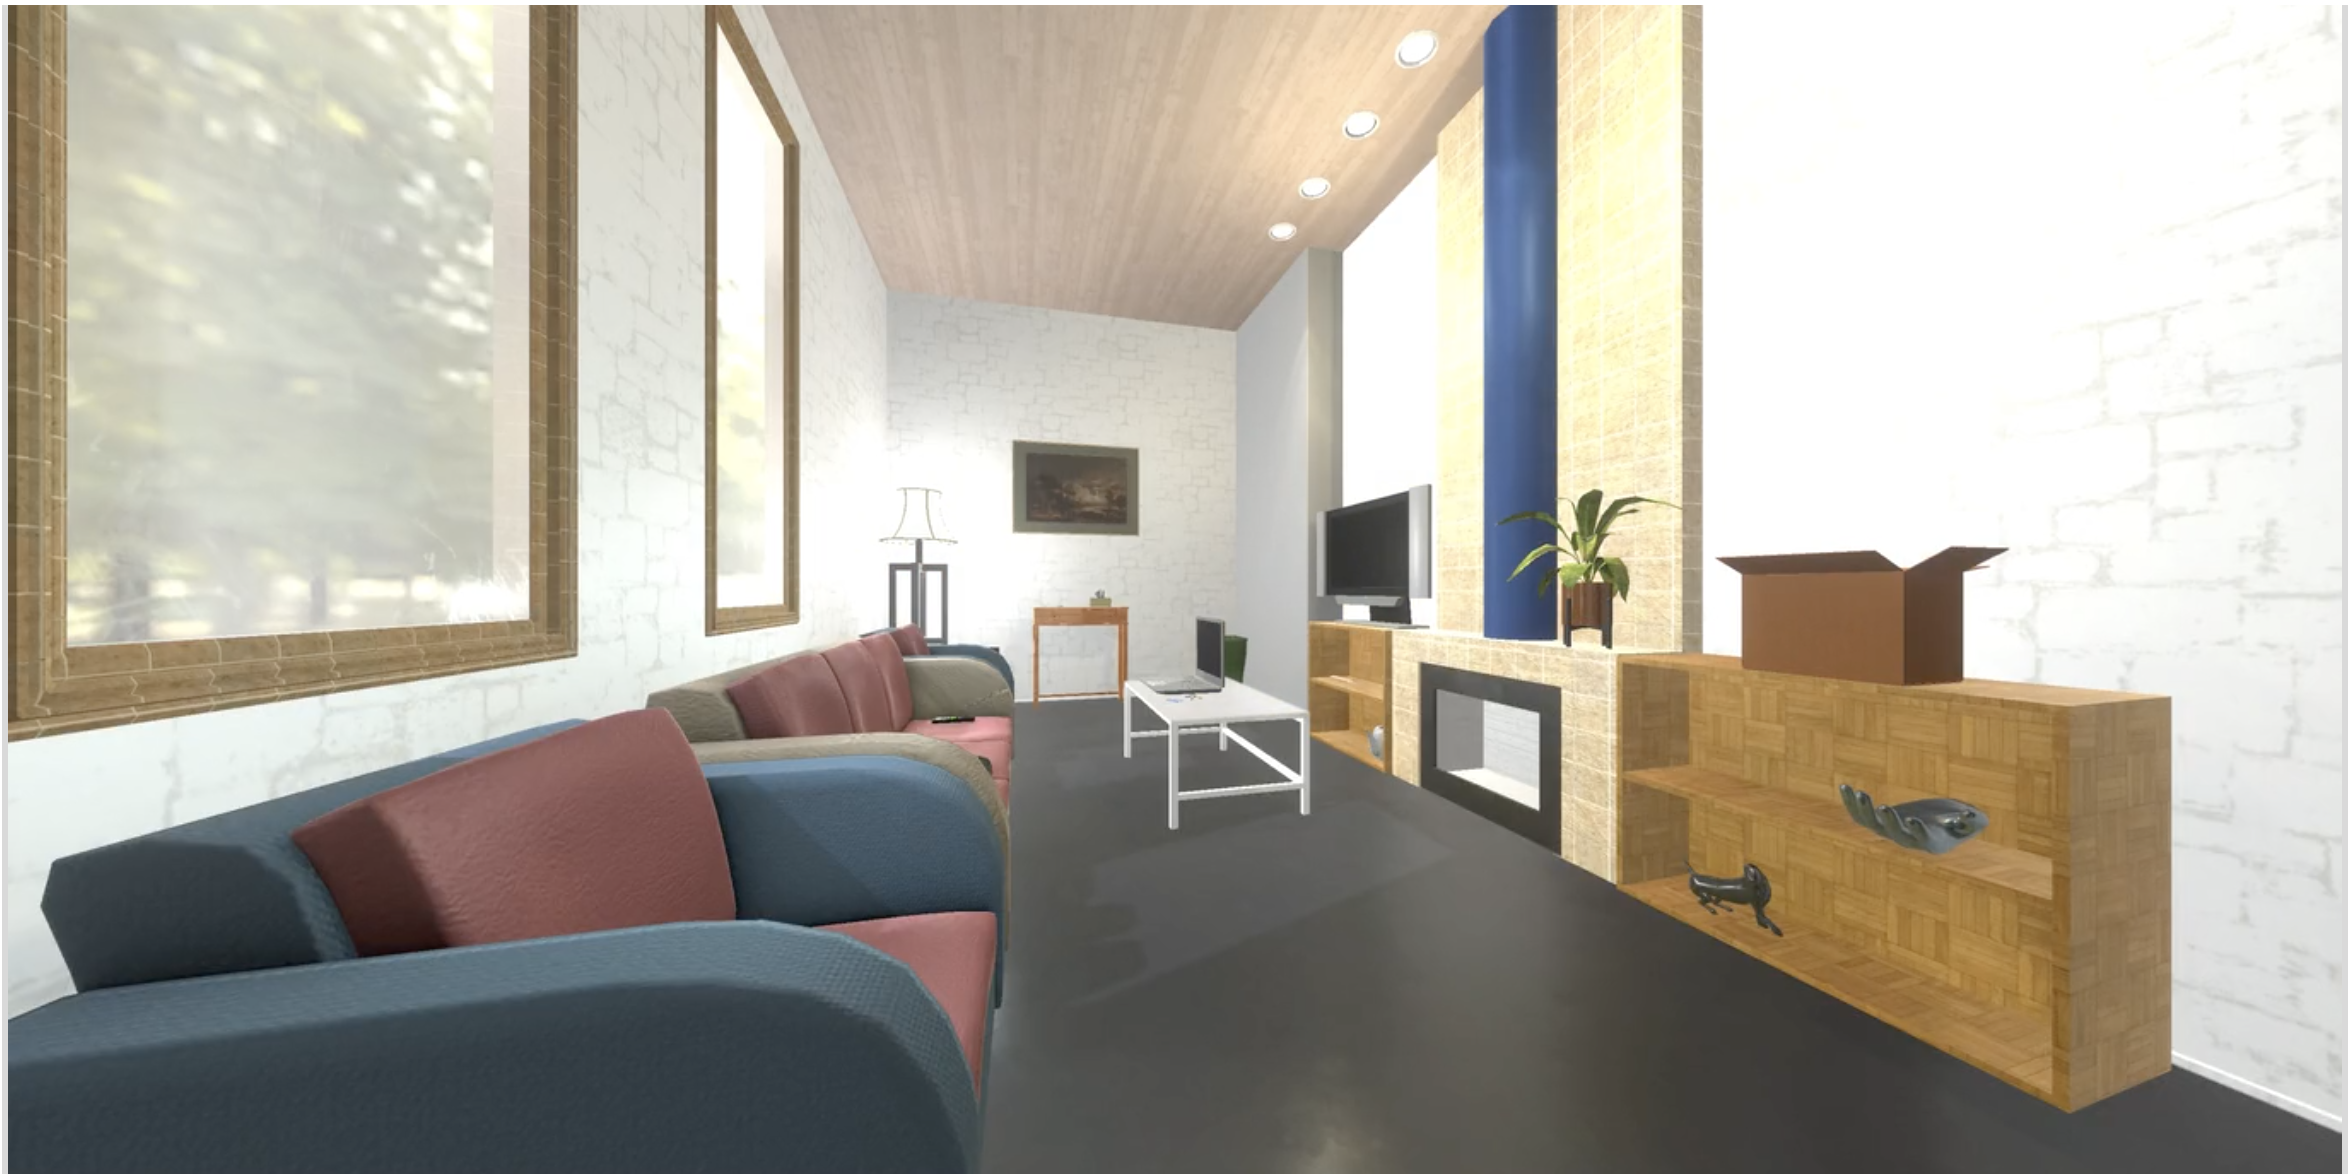
\includegraphics[width=.2\linewidth,valign=m]{/Users/apple/OVGU/Thesis/code/3dReconstruction/report/images/realistic_images_relatedwork/ai2thor_01} &
    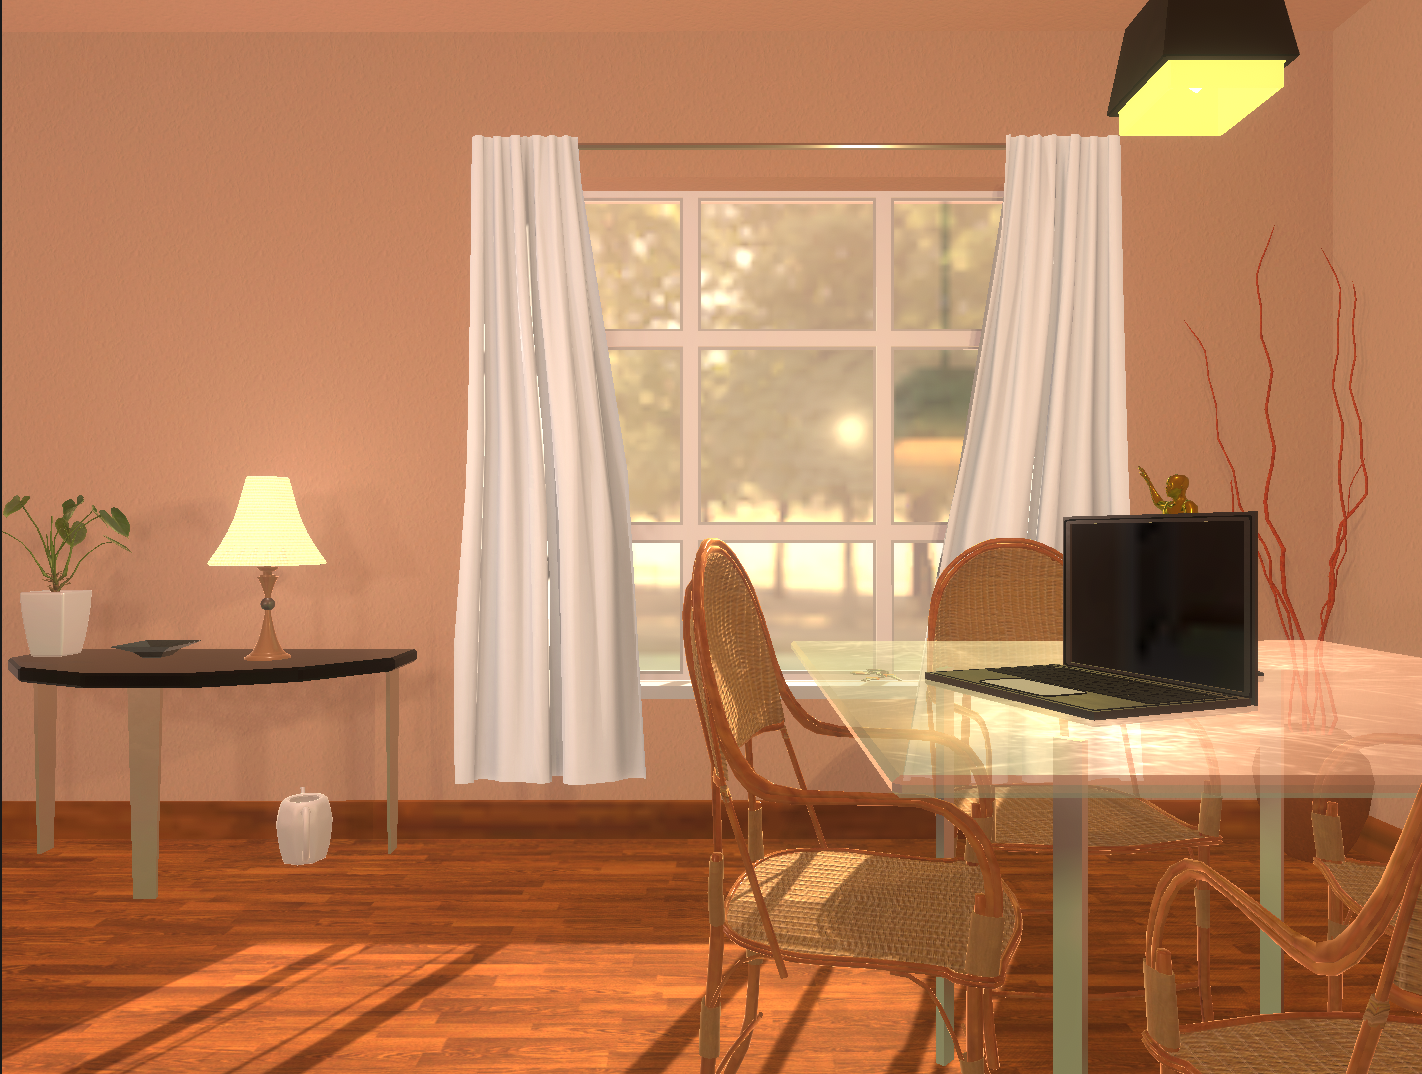
\includegraphics[width=.2\linewidth,valign=m]{/Users/apple/OVGU/Thesis/code/3dReconstruction/report/images/realistic_images_relatedwork/ai2thor_02} &
    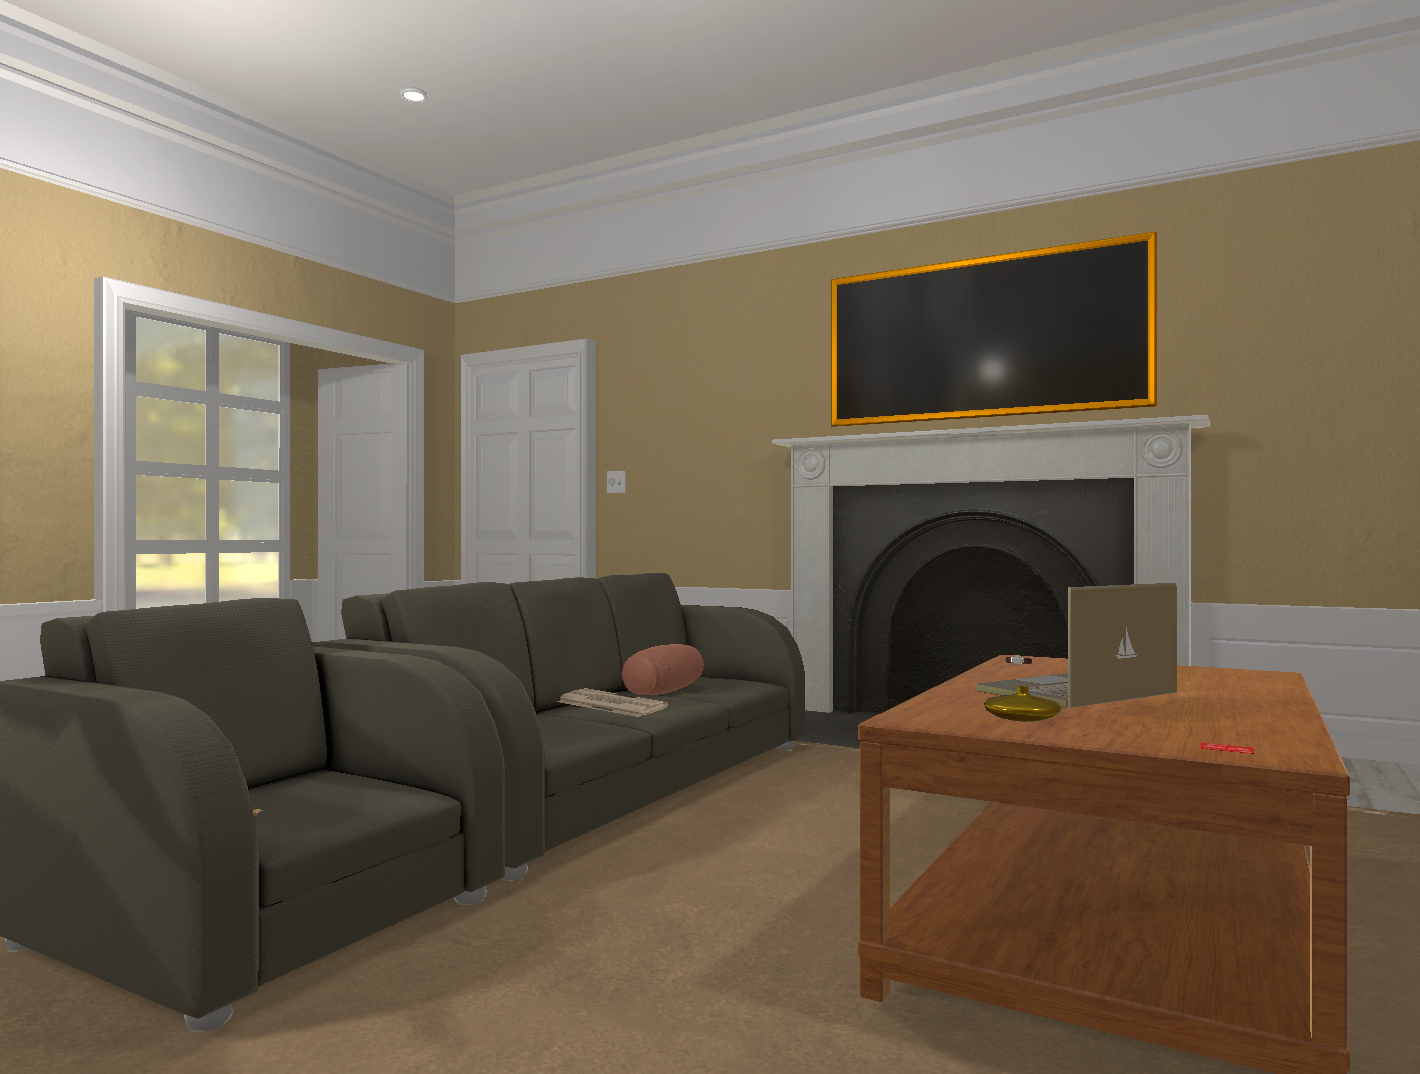
\includegraphics[width=.2\linewidth,valign=m]{/Users/apple/OVGU/Thesis/code/3dReconstruction/report/images/realistic_images_relatedwork/ai2thor_03}\\

    Hypersim & 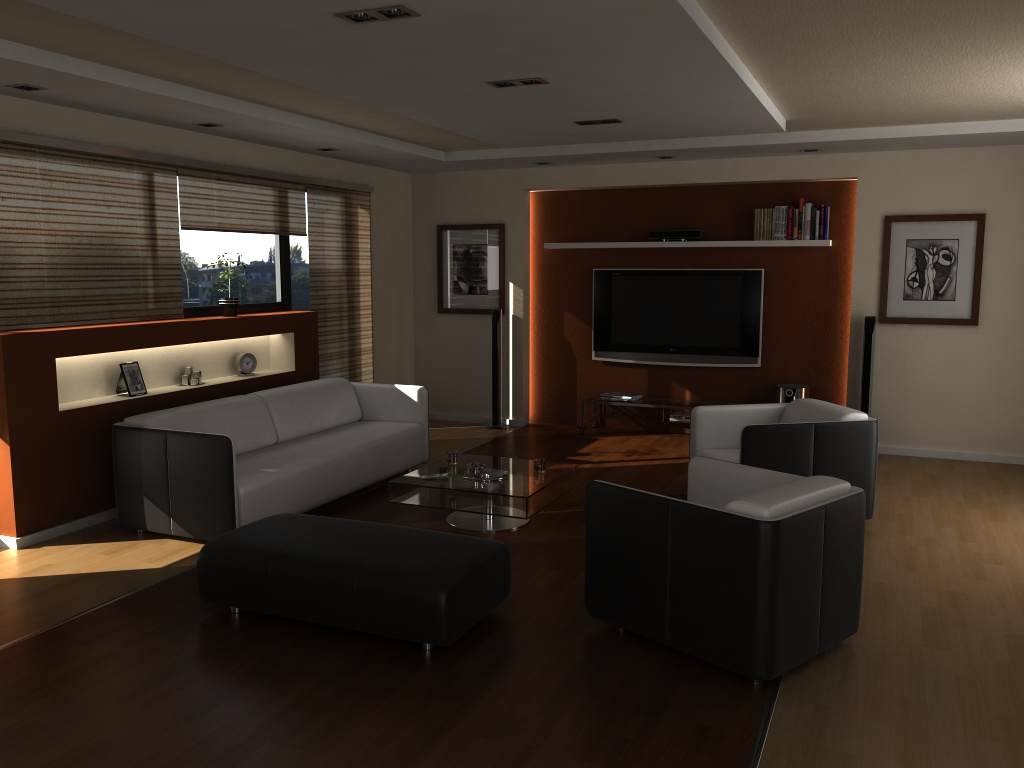
\includegraphics[width=.2\linewidth,valign=m]{/Users/apple/OVGU/Thesis/code/3dReconstruction/report/images/realistic_images_relatedwork/hypersim_01} &
    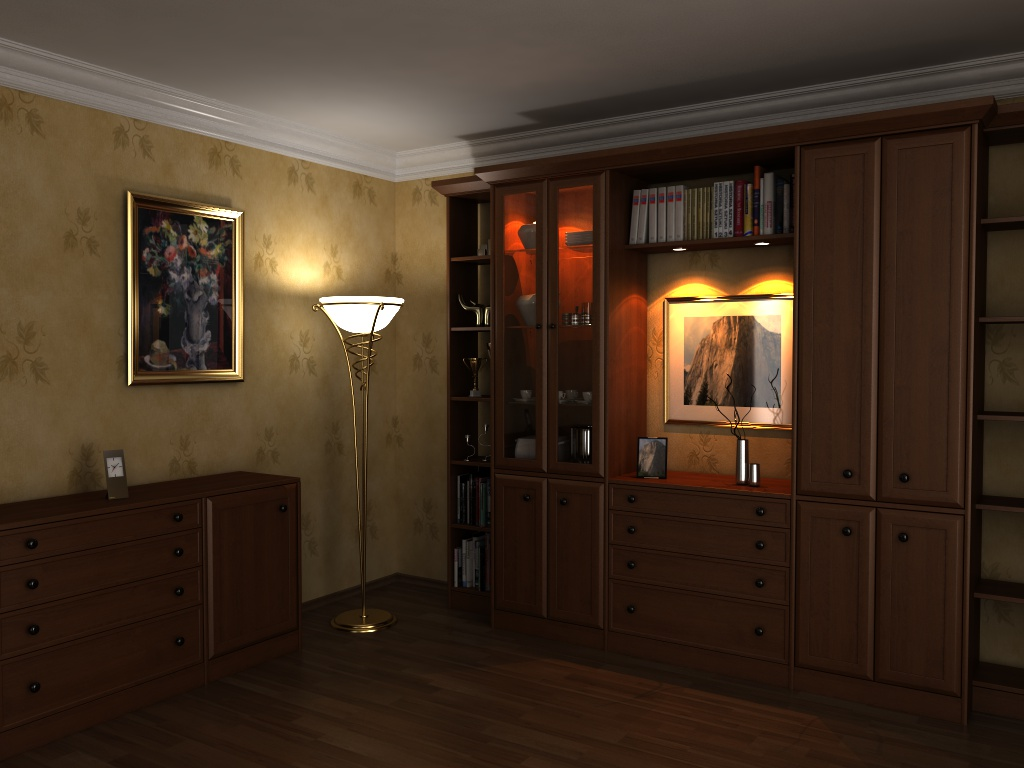
\includegraphics[width=.2\linewidth,valign=m]{/Users/apple/OVGU/Thesis/code/3dReconstruction/report/images/realistic_images_relatedwork/hypersim_02} &
    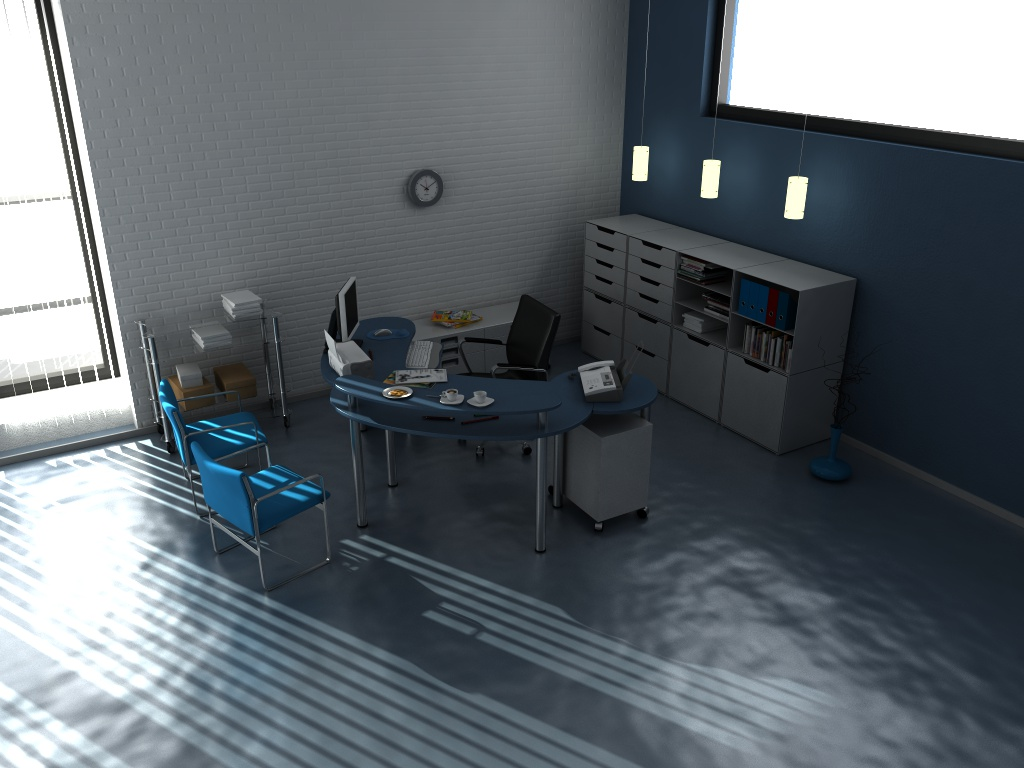
\includegraphics[width=.2\linewidth,valign=m]{/Users/apple/OVGU/Thesis/code/3dReconstruction/report/images/realistic_images_relatedwork/hypersim_03}\\

    InteriorNet & 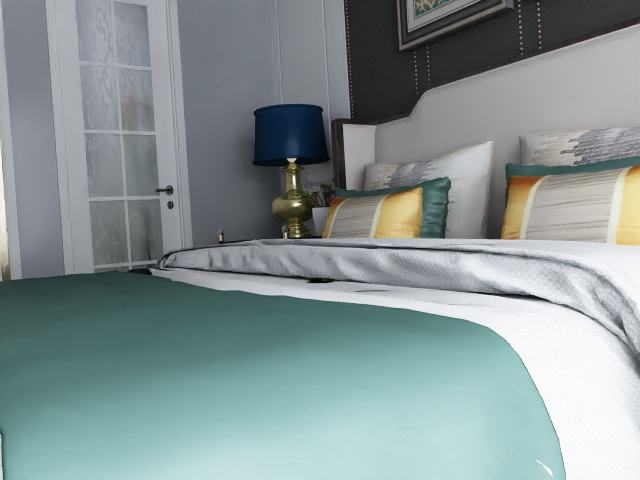
\includegraphics[width=.2\linewidth,valign=m]{/Users/apple/OVGU/Thesis/code/3dReconstruction/report/images/realistic_images_relatedwork/interiornet_01} &
    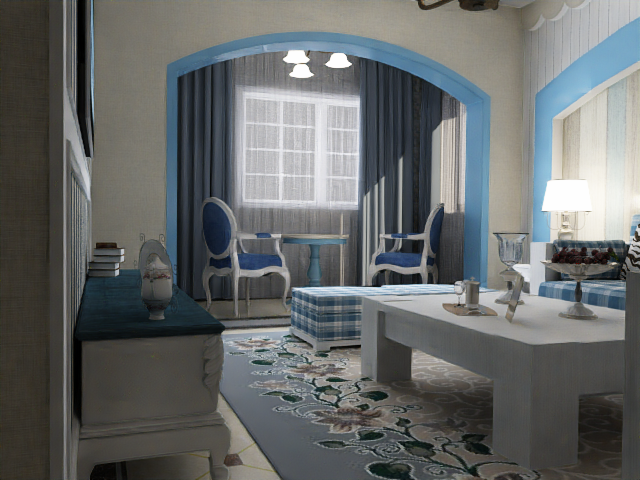
\includegraphics[width=.2\linewidth,valign=m]{/Users/apple/OVGU/Thesis/code/3dReconstruction/report/images/realistic_images_relatedwork/interiornet_02} &
    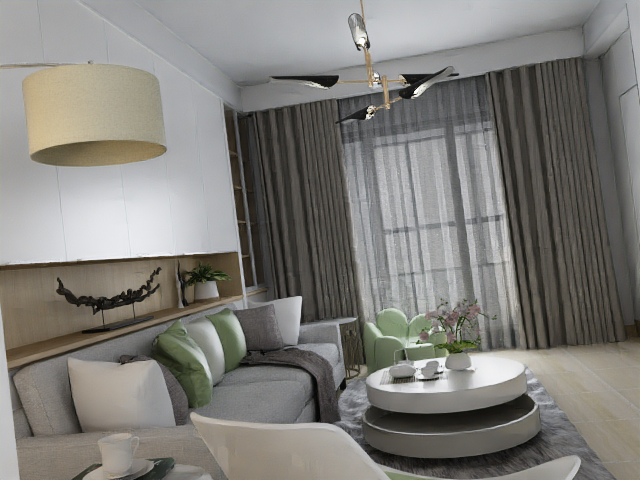
\includegraphics[width=.2\linewidth,valign=m]{/Users/apple/OVGU/Thesis/code/3dReconstruction/report/images/realistic_images_relatedwork/interiornet_03}\\

    OpenRooms & 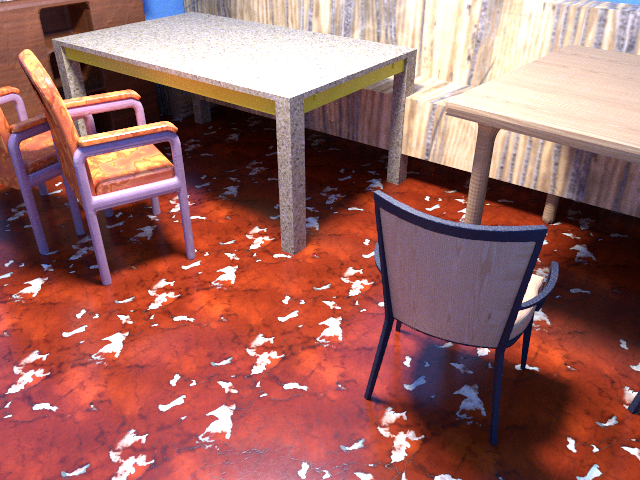
\includegraphics[width=.2\linewidth,valign=m]{/Users/apple/OVGU/Thesis/code/3dReconstruction/report/images/realistic_images_relatedwork/openrooms_01} &
    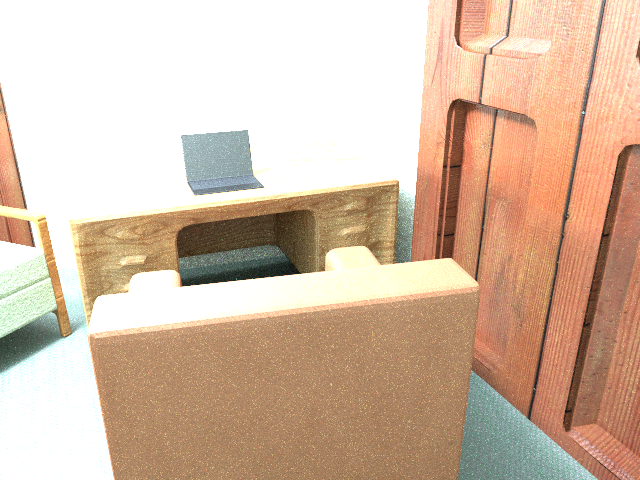
\includegraphics[width=.2\linewidth,valign=m]{/Users/apple/OVGU/Thesis/code/3dReconstruction/report/images/realistic_images_relatedwork/openrooms_02} &
    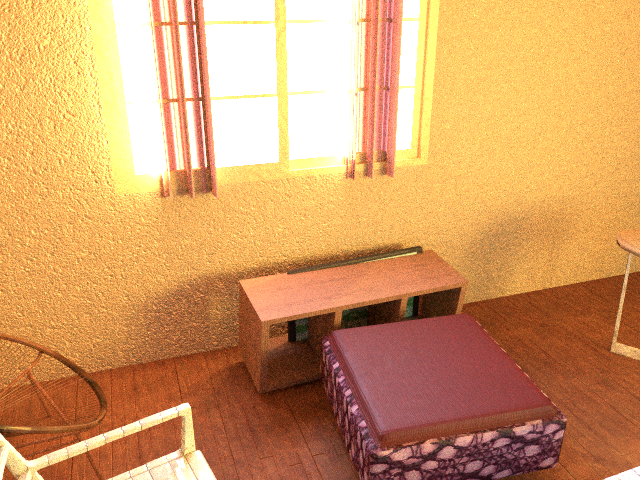
\includegraphics[width=.2\linewidth,valign=m]{/Users/apple/OVGU/Thesis/code/3dReconstruction/report/images/realistic_images_relatedwork/openrooms_03}\\

    SceneNet & 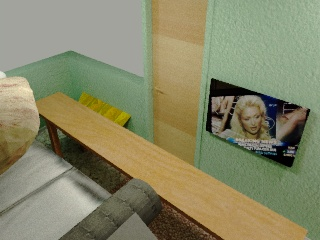
\includegraphics[width=.2\linewidth,valign=m]{/Users/apple/OVGU/Thesis/code/3dReconstruction/report/images/realistic_images_relatedwork/scenenet_1} &
    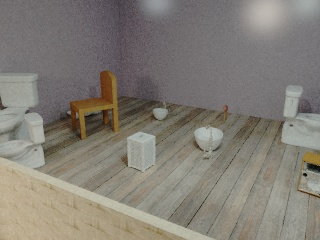
\includegraphics[width=.2\linewidth,valign=m]{/Users/apple/OVGU/Thesis/code/3dReconstruction/report/images/realistic_images_relatedwork/scenenet_2} &
    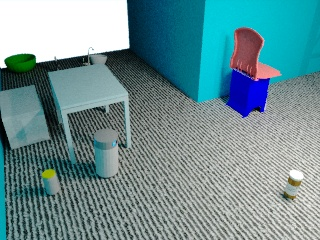
\includegraphics[width=.2\linewidth,valign=m]{/Users/apple/OVGU/Thesis/code/3dReconstruction/report/images/realistic_images_relatedwork/scenenet_3}\\

\end{tabular}
\caption{A collection of photorealistic synthetic datasets. The first column of each row indicates the dataset name followed by randomly selected images from the same dataset.}
\label{fig:photorealistic images comparison}
\end{figure}

\subsection{Tools to create synthetic datasets}\label{subsec:tools-to-create-synthetic}

"BlenderProc: Reducing the Reality Gap with Photorealistic Rendering" by ~\cite{denninger2019blenderproc} is a python based pipeline to create a synthetic dataset.
As the name suggests, the underlying framework is Blender~\cite{blender}, which is a 3D modeling and rendering package.
Like most synthetic data generation tools, it provides RGB, depth maps, normals, and semantic segmentation.
\autoref{fig:Blenderproc samples} is a collection of sample images generated using BlenderPoc.
We searched for synthetic data generation tools, Blenderproc supports a maximum number of existing datasets.
Ikea~\cite{Lim2013ParsingIO}, Pix3d~\cite{pix3d}, Shapenet~\cite{chang2015shapenet}, \gls{front}~\cite{Fu20203DFRONT3F}, Replica~\cite{Straub2019TheRD}, SunCG~\cite{Xiao2013SUN3DAD} are some of the popular datasets it supports.
It also has some combinations of these datasets like ShapeNet with SunCG or SceneNet.
Even though it supports the rendering of the Pix3D dataset, the model is rendered without any background.
One extreme advantage of this toolkit is that it is open source and a more comprehensive open community to contribute.

\begin{figure}
    \begin{tabular}{llll}
        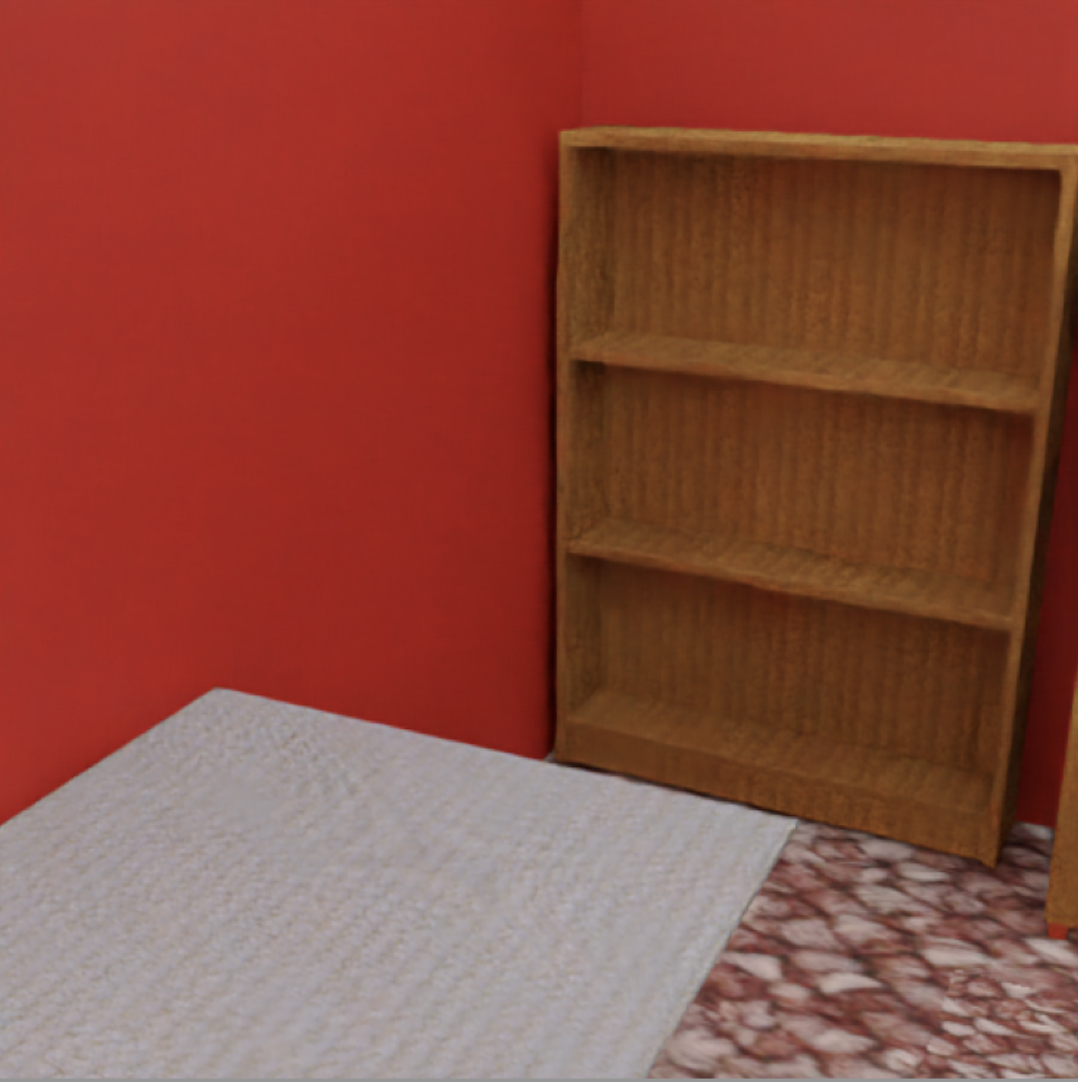
\includegraphics[width=.2\linewidth,valign=m]{/Users/apple/OVGU/Thesis/code/3dReconstruction/report/images/realistic_images_relatedwork/blenderproc_1} &
        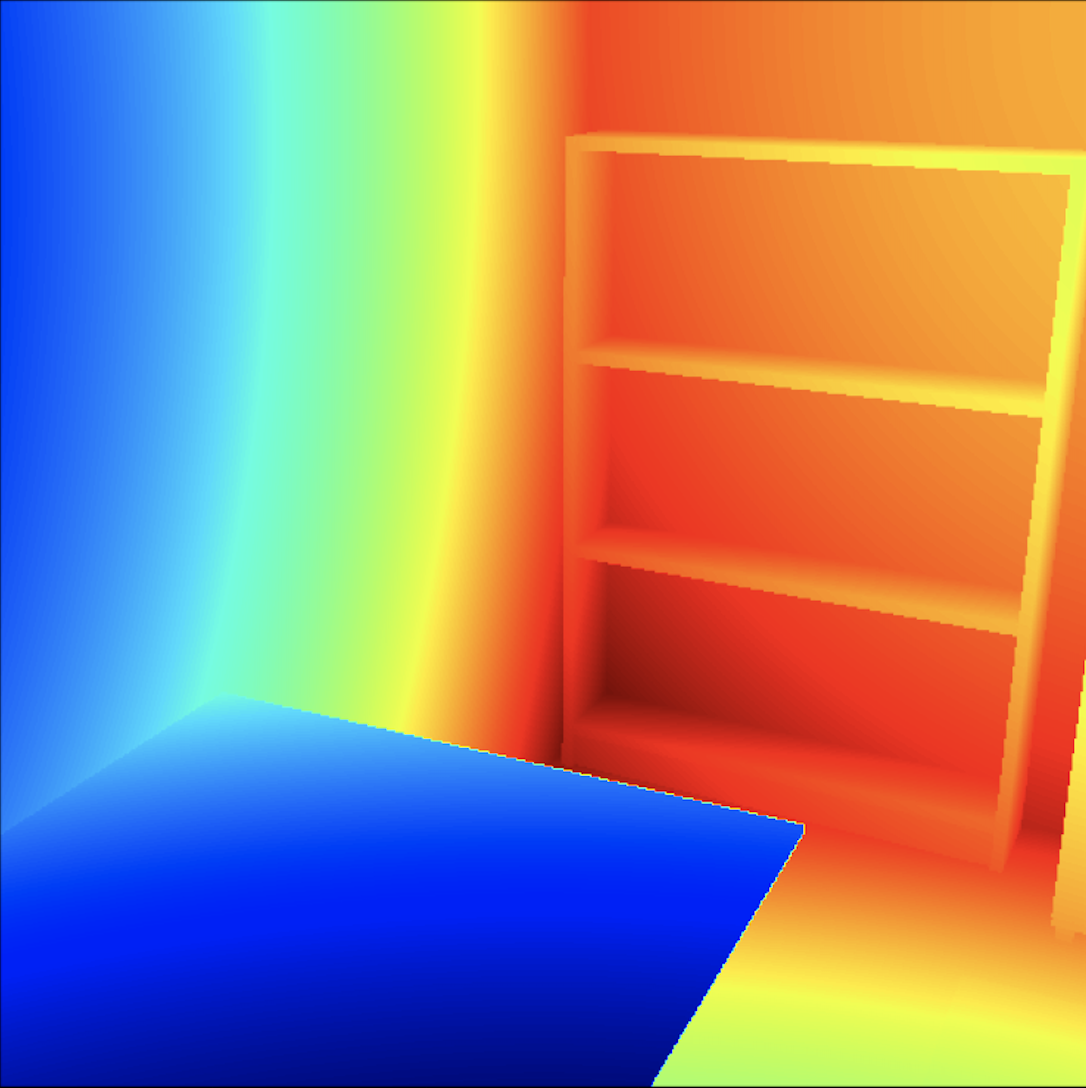
\includegraphics[width=.2\linewidth,valign=m]{/Users/apple/OVGU/Thesis/code/3dReconstruction/report/images/realistic_images_relatedwork/blenderproc_depth_1} &
        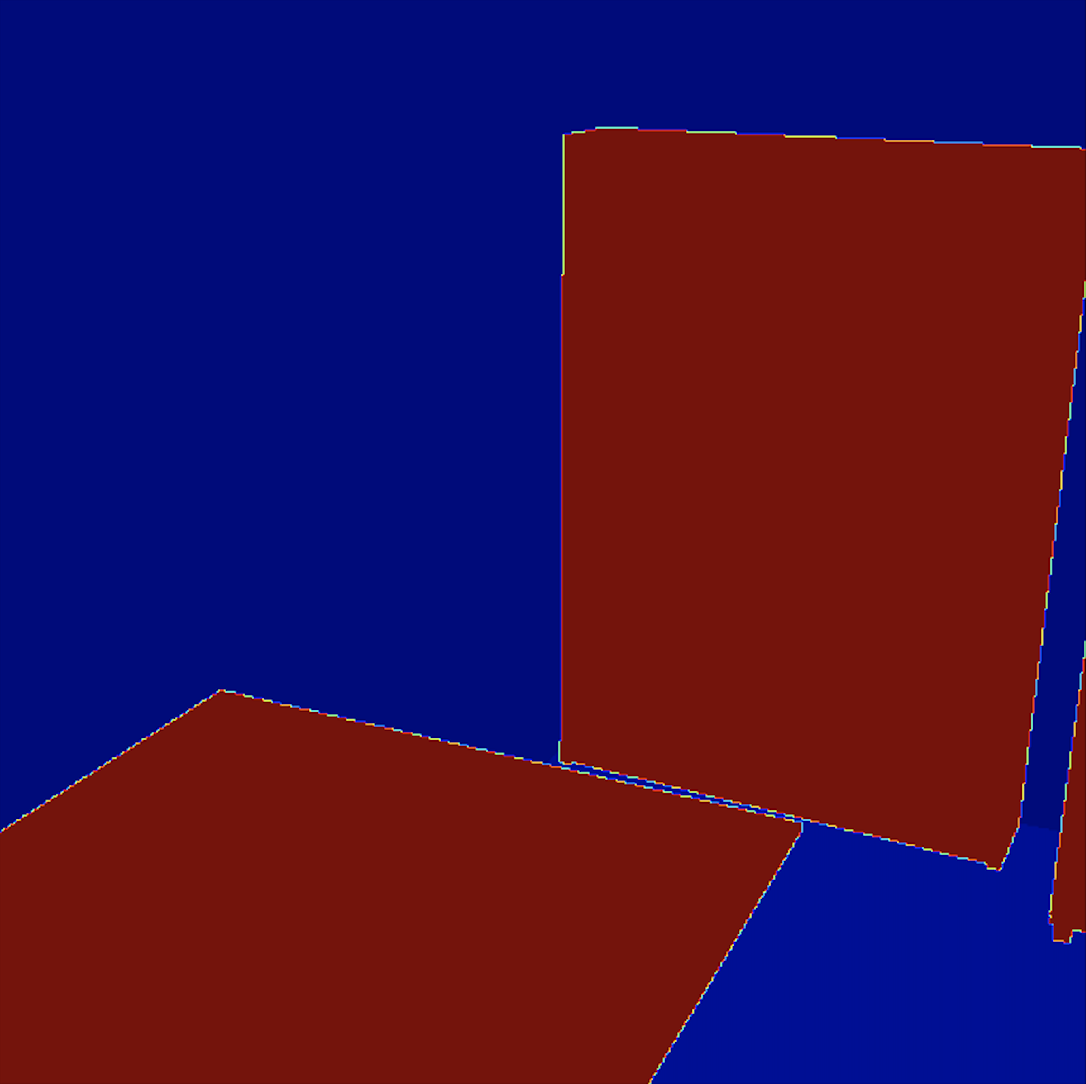
\includegraphics[width=.2\linewidth,valign=m]{/Users/apple/OVGU/Thesis/code/3dReconstruction/report/images/realistic_images_relatedwork/blenderproc_instance_1} &
        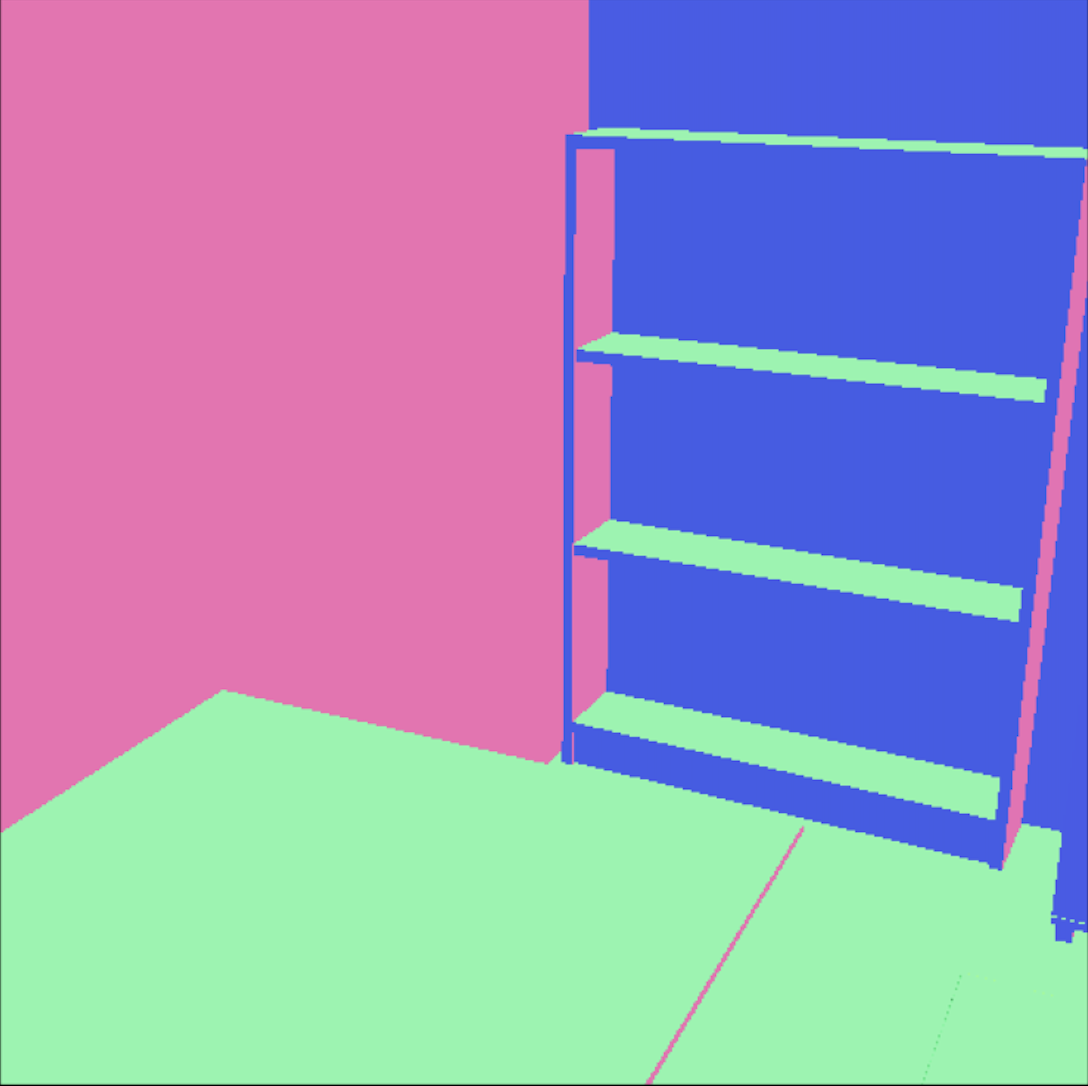
\includegraphics[width=.2\linewidth,valign=m]{/Users/apple/OVGU/Thesis/code/3dReconstruction/report/images/realistic_images_relatedwork/blenderproc_normal_1}\\


        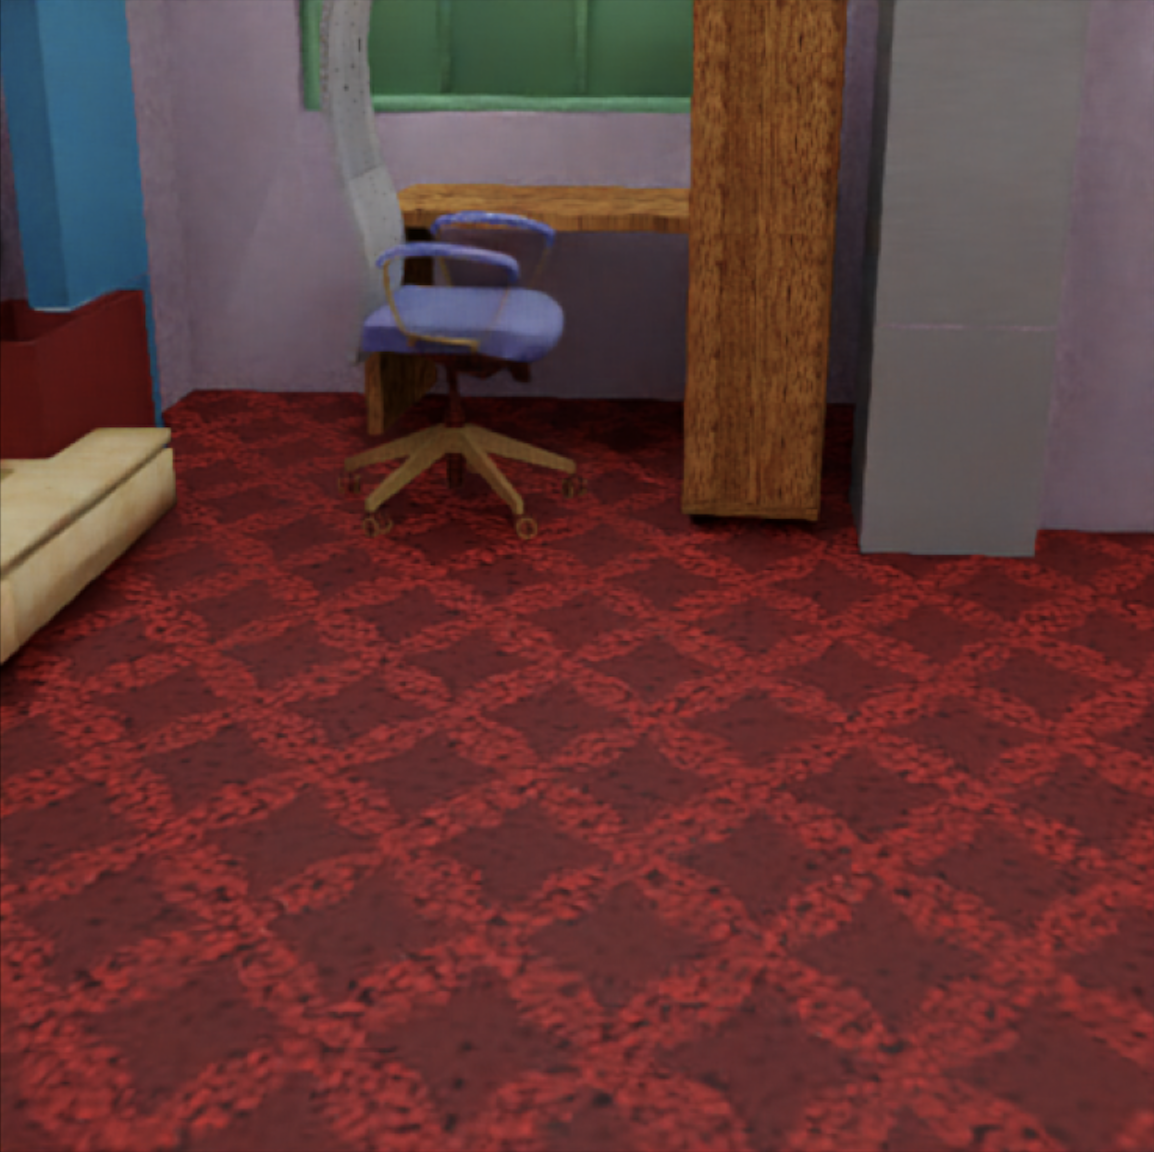
\includegraphics[width=.2\linewidth,valign=m]{/Users/apple/OVGU/Thesis/code/3dReconstruction/report/images/realistic_images_relatedwork/blenderproc_2} &
        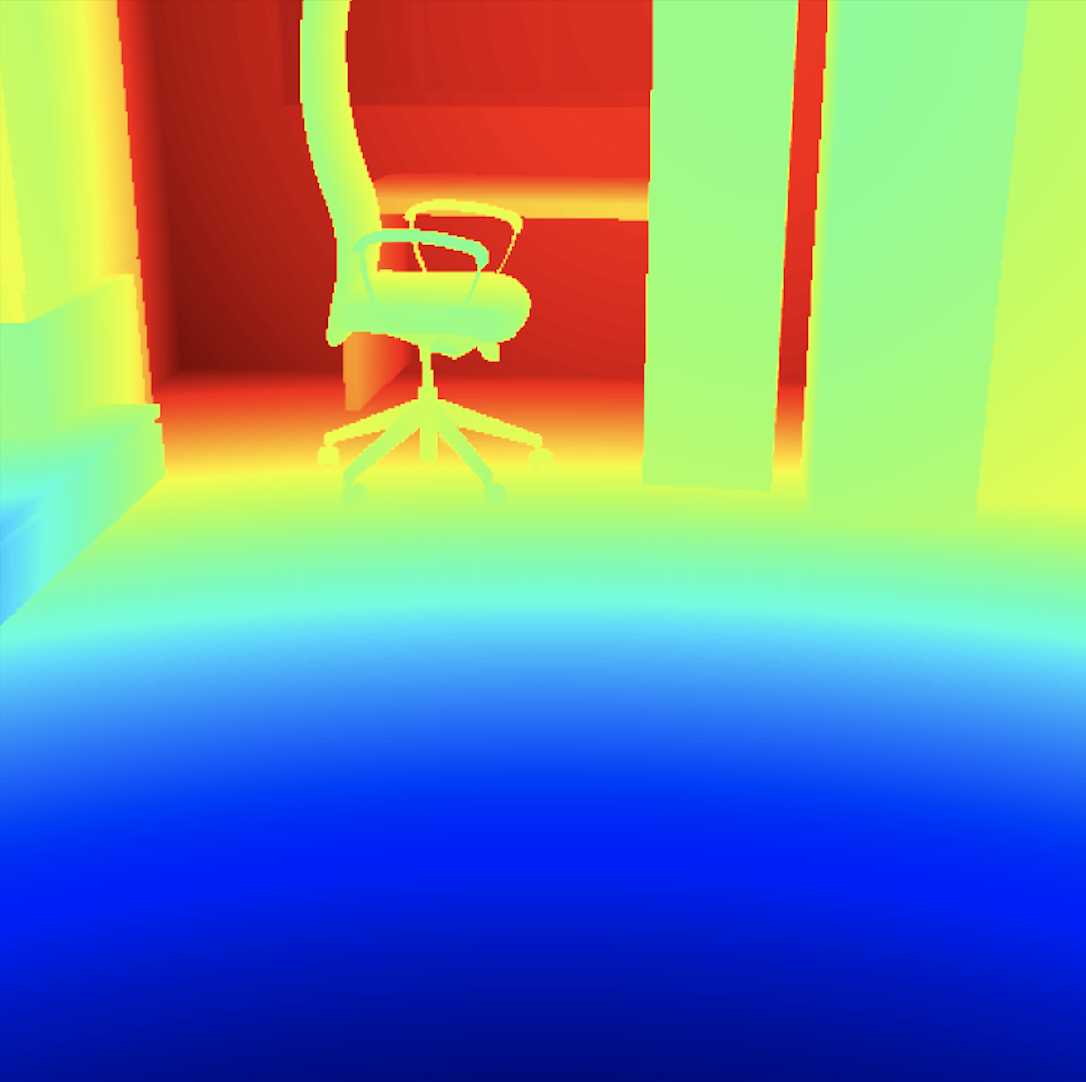
\includegraphics[width=.2\linewidth,valign=m]{/Users/apple/OVGU/Thesis/code/3dReconstruction/report/images/realistic_images_relatedwork/blenderproc_depth_2} &
        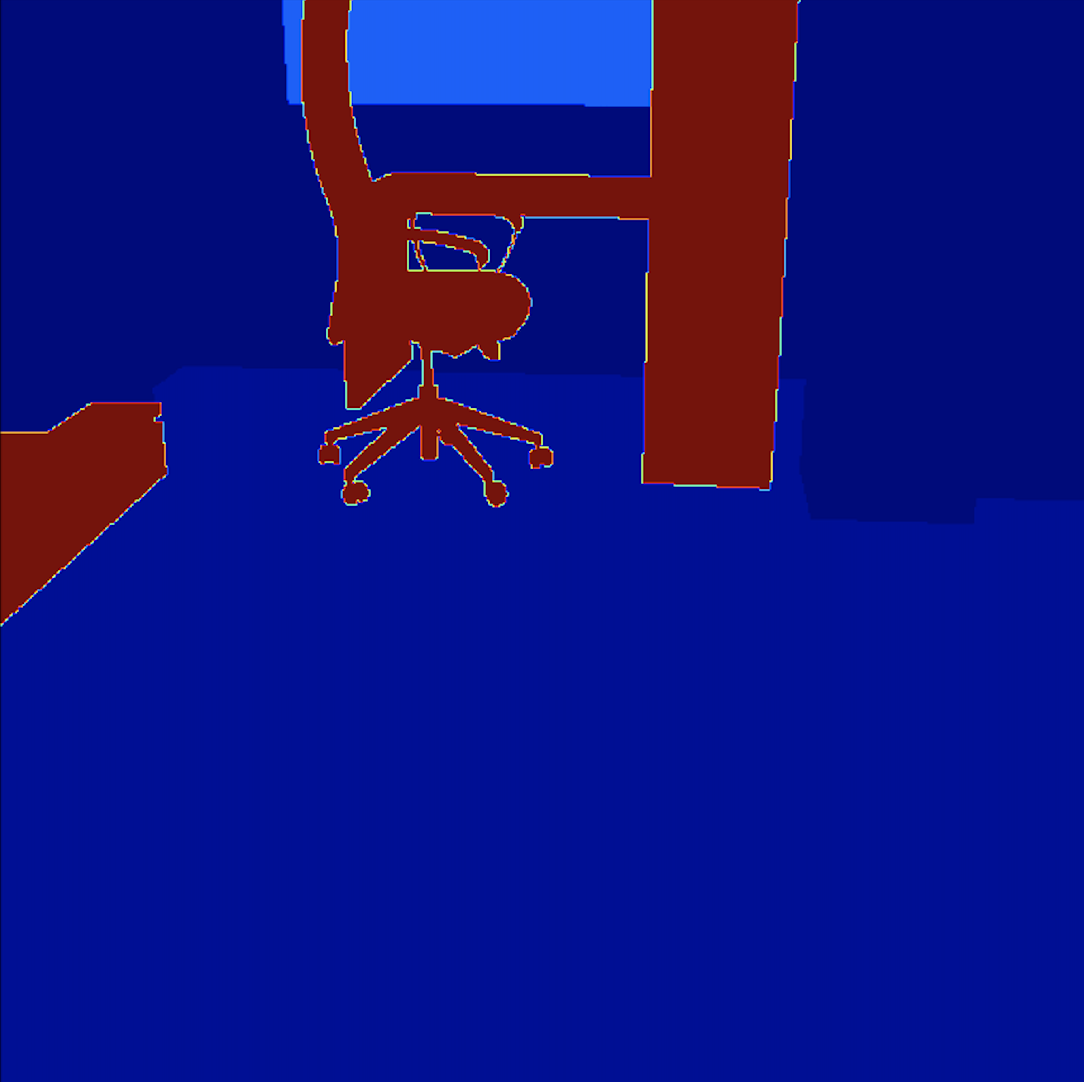
\includegraphics[width=.2\linewidth,valign=m]{/Users/apple/OVGU/Thesis/code/3dReconstruction/report/images/realistic_images_relatedwork/blenderproc_instance_2} &
        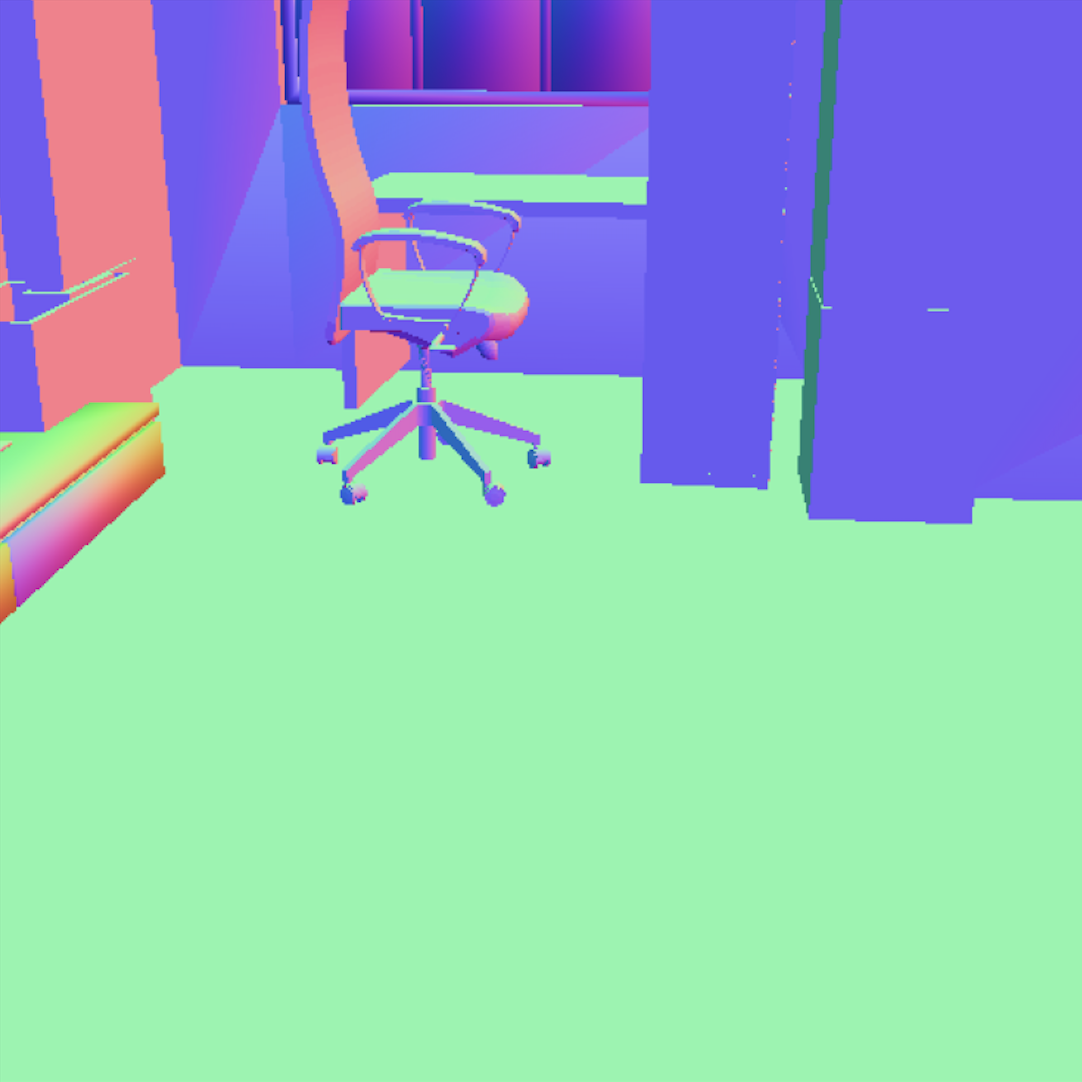
\includegraphics[width=.2\linewidth,valign=m]{/Users/apple/OVGU/Thesis/code/3dReconstruction/report/images/realistic_images_relatedwork/blenderproc_normal_2}\\

%        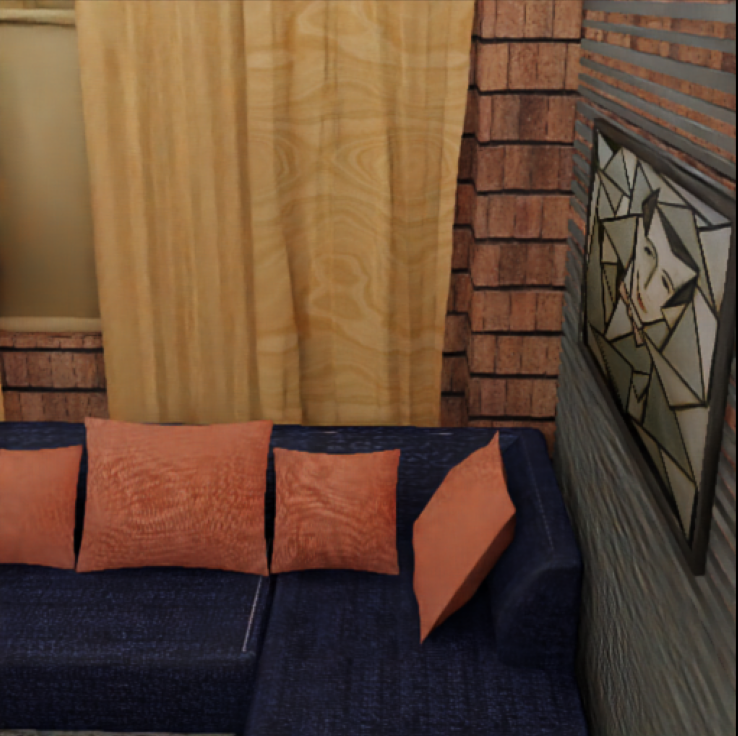
\includegraphics[width=.2\linewidth,valign=m]{/Users/apple/OVGU/Thesis/code/3dReconstruction/report/images/realistic_images_relatedwork/blenderproc_3} &
%        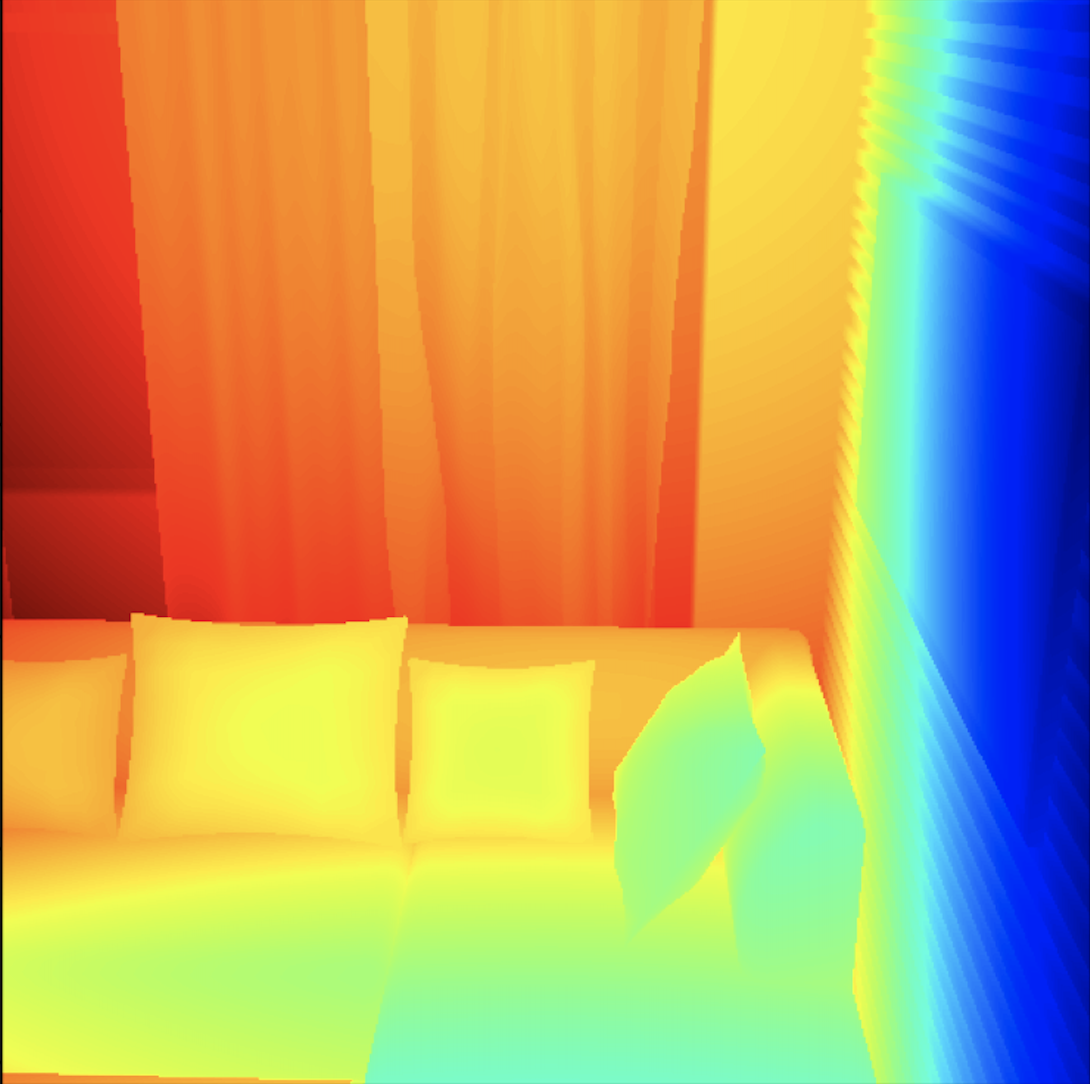
\includegraphics[width=.2\linewidth,valign=m]{/Users/apple/OVGU/Thesis/code/3dReconstruction/report/images/realistic_images_relatedwork/blenderproc_depth_3} &
%        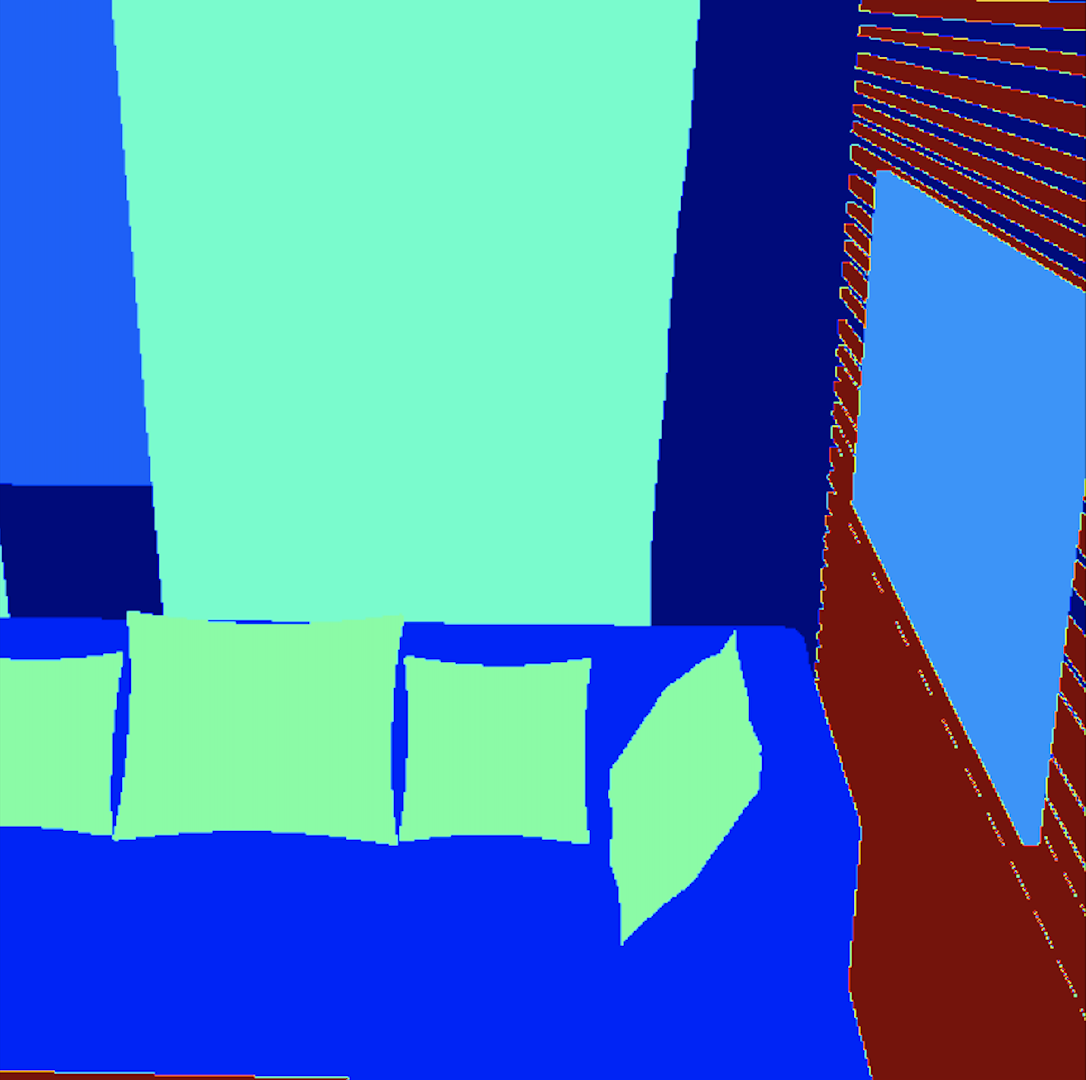
\includegraphics[width=.2\linewidth,valign=m]{/Users/apple/OVGU/Thesis/code/3dReconstruction/report/images/realistic_images_relatedwork/blenderproc_instance_3} &
%        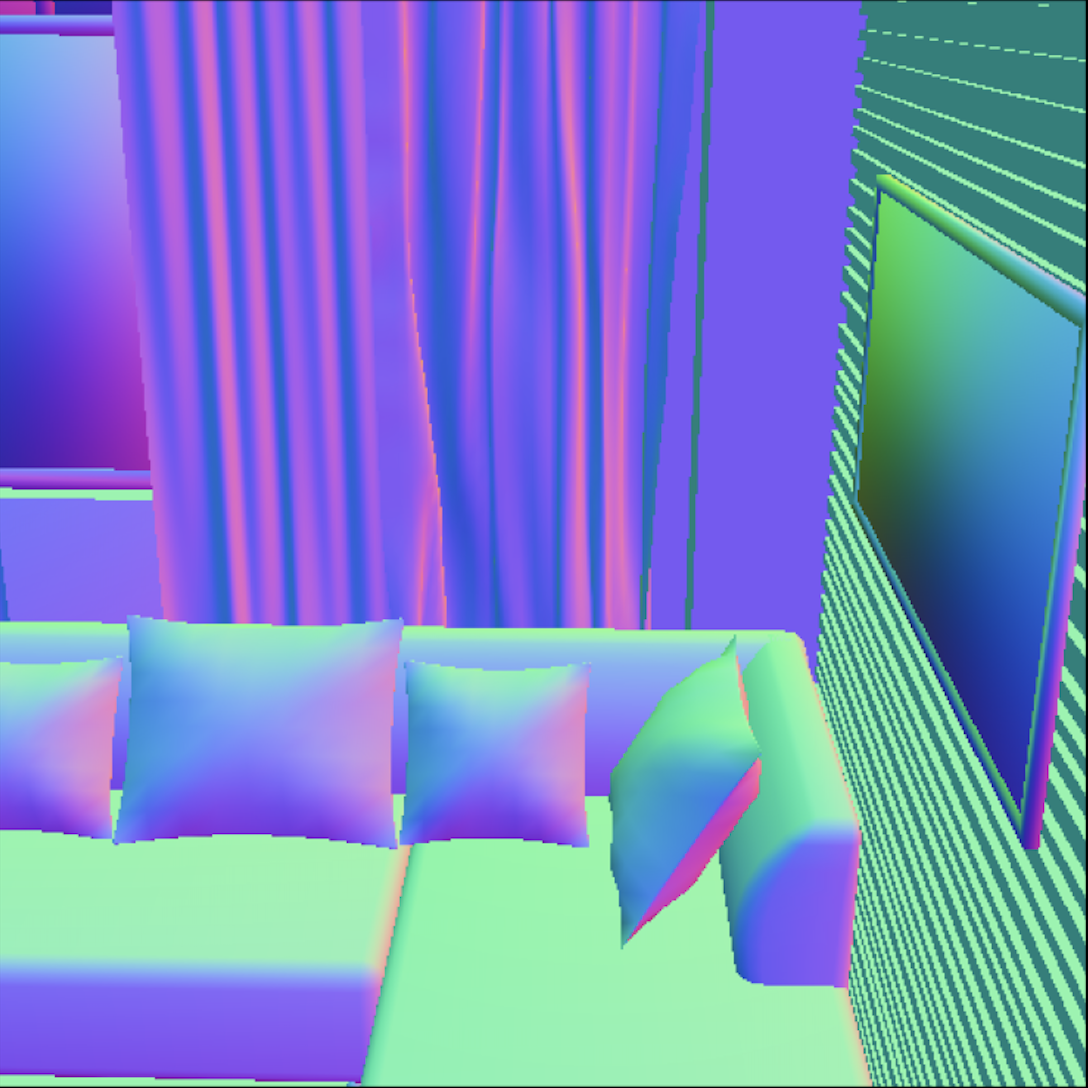
\includegraphics[width=.2\linewidth,valign=m]{/Users/apple/OVGU/Thesis/code/3dReconstruction/report/images/realistic_images_relatedwork/blenderproc_normal_3}\\

    \end{tabular}
    \caption{Sample images created from BlenderProc using SceneNet dataset.(Left to right) RGB images, Depth Maps, Instance Segmenatations and Normals. Each row is an independent sample.}
    \label{fig:Blenderproc samples}
\end{figure}

NVIDIA developed a Deep learning Dataset Synthesizer (NDDS)~\cite{to2018ndds} in the form of a plugin for Unreal Engine 4(UE4).
The plugin can synthesize images, per-pixel segmentation, depth, object 3D pose, 2D/3D bounding box, keypoints, and custom stencils.
It even supports domain randomization of objects, lighting, camera position, poses, and textures.
They Leveraged the asynchronous, multithreaded frames to generate data at high rates(50-100 Hz) for Falling Things (FAT)~\cite{tremblay2018falling} dataset.

"SynthDet: An end-to-end object detection pipeline using synthetic data"~\cite{synthdet2020} is an open-source project supported by Unity technologies using Unity Engine.
This ML pipeline uses 63 everyday objects(example: cereal box, cady, cartons, and more) as synthetic objects to generate 2D bounding boxes.
This project was highly influenced by~\cite{hinterstoisser2019annotation}, wherein they used synthetic 3D models with a randomized background to generate a synthetic dataset for the object detection task.
With domain randomization, the author of~\cite{hinterstoisser2019annotation} proved that no real data or mixed training is required for the Deep Learning model to perform significantly.

UnrealCV~\cite{qiu2017unrealcv} is an open-source project built upon Unreal Engine 4 (UE4)~\cite{unrealengine}).
It supports some pre-built indoor architectures available on the asset store, which are unfortunately paid versions.
Along with this limitation, the plugin only creates depth maps, normals, and segmentation masks, with no mapping to 3D models.
Another tool based on the Unreal engine is UnrealROX+\cite{martinezgonzalez2021unrealrox}.
This plugin design is based on UnrealCV and provides similar data.

\section{State of the art for 3d-reconstruction}\label{sec:state_of_the_art}

3D reconstruction task is on the rise with improvements in technologies like Augmented and virtual reality.
Scene understanding becomes essential for these technologies to succeed.
As discussed in \autoref{sec:Volumetric representation}, 3D models have voxels, meshes, and point clouds as representations.
Each of the representations has been explored for reconstruction, and this section explores some approaches.

The task can either be applied to \b{a multi-view, or a single view image}.
~\cite{Kar2017LearningAM, choy20163d, Yang_2019, huang2018deepmvs, Paschalidou2018RayNetLV, Xie_2019, Xie_2020},
are architectures based on multiple input images of the same images from different views to learn the underlying 3D structure.
~\cite{Kar2017LearningAM, choy20163d} are architectures based on Recurrent Neural Networks (\gls{rnn}) and have the disadvantage of memory,
long-term dependencies, and long inference time.
~\cite{Yang_2019, huang2018deepmvs, Paschalidou2018RayNetLV} explore different ways of pooling(attentional, max, and average pooling, respectively)
to aggregate the feature vectors from different views.
The pooling method tends to capture only partial information with loss in detail.

For single-view reconstruction, we have architectures like~\cite{wu2017marrnet,z-gan, Yang_219, wu2018learning, popov2020corenet}.
~\cite{wu2017marrnet} predict the 3D structure by estimating 2.5D properties like surface normals, segmentation, and depths.
~\cite{wu2018learning} is an extension of MarrNet, which proposes a network to preserve the naturalness of the surface.
Inspired by generative models~\cite{Goodfellow2014GenerativeAN,kingma2014autoencoding}, many 3D reconstruction architectures were published~\cite{z-gan, Yang_219,wu2017learning,Lunz2020InverseGG}.
Both~\cite{Xie_2019, Xie_2020} also can predict 3D structure from a single view image.

Many new architectures have also been proposed to overcome the memory issues caused by 3D voxels~\cite{tatarchenko2017octree,Richter2018MatryoshkaNP,Mescheder2019OccupancyNL,Gkioxari2019MeshR, wang2018pixel2mesh,groueix2018atlasnet,pan2019deep}.
These are approaches that are based out of oct-tree, meshes, occupancy of a voxel.
Occupancy networks are an implicit way of representing 3D surfaces as decision boundaries using the network as a deep learning classifier.
For mesh-based reconstruction, a template mesh such as an ellipsoid is deformed to get the structure of the 3D model.
For the Oct-tree-based reconstruction, as the name suggest, instead of 3D voxels, the models are discretized in Oct-Tree representation.
Oct-tree can further make the process memory and compute efficient, providing higher resolution than 3D voxel representation.

Supervision is another factor to consider for 3D reconstruction tasks.
There are methods based on \b{3D-Supervision or 2D-Supervision}.
~\cite{Xie_2019,Xie_2020,wu2017marrnet,groueix2018atlasnet,pan2019deep, chen2019learning} are few of the 3D-supervision based architecture.
For all these architectures, it is necessary to either have the 3D voxel grid or 3D mesh for supervised training.
For models described in~\cite{Lunz2020InverseGG,henderson2019learning},the 3D reconstruction only needs 2D supervision like a silhouette.
One might argue that for 3D supervision, we need a large number of 3D models designed and created by professional artists
With the advent of Virtual and Augmented realities, 3D models available to the public is increasing exponentially, which might resolve the issue.

\section{Mitigating domain shift}\label{sec:mitigating_domain_shift}

The idea of domain randomization is that real images appear to be one of the many variations among training images from synthetic datasets.
Thus, testing with real-world images should give a comparable performance.
~\cite{tobin2017domain} used this principle for small objects detection tasks used for robotics.
This paper tries different parameters in domain randomization like lights, camera viewpoints, and textures and combines domain randomization with domain adaptation.

~\cite{prakash2020structured} introduced Structured domain randomisation, where the structure and context are preserved for the problem while creating synthetic images.
Example: A road is randomly placed with parameters like curvature, lighting, and camera position.
With this as context, they generate pedestrian walk, road lanes, etc.
After these two steps, the objects such as cars, cyclists, houses, buildings are placed on the scene.
As an ablation study, the author changes domain randomization parameters and checks the performance of the car detection task.

~\cite{georgakis2017synthesizing} proposed domain randomization-based synthetic images generation to detect objects found in the kitchen.
The objects are cropped and placed on the background with semantic information and geometry with proper scale.
Similar to the above works, the author also provides an ablation study with different ratios of synthetic to the real dataset for mixed training.

Domain randomization and adaptation techniques are not the only ways to mitigate the domain shift.
With the advent of Generative Adversarial Networks~\cite{Goodfellow2014GenerativeAN},synthetic to real image conversions have become possible and lead to better performance on given tasks.
~\cite{Richter_2021, CycleGAN2017, park2020cut,isola2017image, dundar2018domain,Wang2018HighResolutionIS} are some successful attempts to reduce the gap between simulated environment and reality.
Intel in~\cite{Richter_2021} uses GTA V dataset with G-buffers(depth, normals, segmentations, Albedo, glossiness, etc.) to enhance the photorealism of synthetic images.
~\cite{park2020cut} use a patchwise contrastive loss to retrain the content of the input image.
They minimize the loss such that corresponding patches retain high mutual values.

Another exciting way to reduce the domain gap is using domain adversarial training~\cite{ganin2016domainadversarial}.
Along with the task under observation, a branched network from the feature extractor is used as a classifier for the domains.
This acts like a multi-learning task where the feature extractor is the common branch.
In one branch the model learns to perform a specific task like segmentation or classification.
The other branch classifies if the dataset is real or synthetic.
~\cite{pinheiro2019domainadaptive} implements the same principle on complex 3D reconstruction tasks by predicting voxels and classifying the image domain.

\subsection{Training with synthetic dataset}\label{subsec:training-with-synthetic-dataset}
The research questions, as stated in \autoref{sec:goal} aims to check if a synthetic dataset can deliver as a standalone dataset.
If it does not, then techniques like fine-tuning will be helpful.
Another way to use the large synthetic datasets is using mixed training.

In~\cite{nowruzi2019real},  the author tries to find how much real data is required with the synthetic dataset to increase the performance of object detection tasks.
A study was conducted by training various object detection models on mixed data containing different real and synthetic datasets ratios.
The four ratios considered for mixed training were 0\%, 90\%, 95\%, 97.5\% of synthetic data to real data.
Another study was conducted by fine-tuning a model pre-trained on a synthetic dataset with real datasets of different sizes.
They observed that fine-tuning with a limited real dataset is better than mixed training with a synthetic dataset.

~\cite{Tremblay2018TrainingDN}  explore domain randomization on real-world object detection.
The author also proposes a new approach of domain randomization, wherein random 3d objects called ”flying distractors” are randomly placed in the scene;
the model learns to ignore objects that are not of interest.
A focused ablation study with individual domain randomization parameters was also conducted to understand the contribution of each component.
The parameters included lights, textures, data augmentation, and flying distractor, as mentioned above.
Also, object detection is trained with varying dataset sizes to learn its impact.
They also conducted a study of the dataset size needed to fine-tune a pre-trained model optimally.

\cite{2018LearningIC} used mixing ratios for classification task for each of the mini-batches and observed 5-13\% improvement in performance.
The mixing ratios used were 1:15, 1:7, and 1:1.
A comprehensive study was made on randomization using datasets containing textures, random camera positions, background, lightings, and augmentations.

